\documentclass[14pt, fleqn, a4paper]{extarticle}
\usepackage{amsmath, amssymb, amsthm} % amsopn, amsfonts
\usepackage[no-math]{fontspec}
\usepackage{enumitem, xparse}
\usepackage[normalem]{ulem}
\usepackage{indentfirst}
\usepackage{polyglossia}
\usepackage{changepage}
\usepackage{geometry}
\usepackage{multicol}
\usepackage{fancyhdr}
\usepackage{multirow}
\usepackage{setspace}
\usepackage{tabularx}
\usepackage{booktabs}
\usepackage{lastpage}
\usepackage{hyperref}
\usepackage{graphicx}
\usepackage{ltablex}
\usepackage{import}
\usepackage{float}
\usepackage{array}

% \import{./}{preamble.sty}

\geometry{
	% a4paper, 
	% paperwidth=210mm,
	% paperheight=297mm,
	top=1in, 
	bottom=1in, 
	left=1in, 
	right=1in
}

\XeTeXlinebreaklocale "th"
\XeTeXlinebreakskip = 0pt plus 0.5pt
\keepXColumns

\setmainfont{TH SarabunPSK}[Scale=1.15]

\defaultfontfeatures{Scale=MatchLowercase,Ligatures=TeX}
\setdefaultlanguage{thai}
\setotherlanguage{english}
\newfontfamily\thaifont[Script = Thai]{TH SarabunPSK}
% \newfontfamily\latinfont{TH SarabunPSK}

% \pagestyle{empty}
\setstretch{1.25}
\setdisplayskipstretch{0.5}
\setlength{\parindent}{2em}
\setlength{\parskip}{0.75em} % 0.5em
\setlength{\mathindent}{0.5in}

\urlstyle{same}
\hypersetup{
    colorlinks = true,
    urlcolor = black,
    linkcolor = black,
    citecolor = black
}

\pagestyle{fancy}
\fancyhf{}
\fancyfoot[C]{หน้า \thepage\ จาก \pageref{LastPage}}
\renewcommand{\headrulewidth}{0pt}
\renewcommand{\footrulewidth}{0pt}

\setlist[enumerate,2]{label=\theenumi.\arabic*.}

% \title{\fontsize{18pt}{20pt}\selectfont \textbf{แบบเสนอโครงงานเทคโนโลยี}}

\makeatletter
\renewcommand{\maketitle}{
	\begin{center}
		\vspace*{-3em}
		{\@title\par}
		\vspace{-1.0em}
		% \rule{0.8\textwidth}{0.5pt}
	\end{center}
}
\makeatother

\makeatletter

\renewcommand\section{%
  \@ifstar{\flatsection}{\@section}%
}

\newcommand{\flatsection}[1]{%
   \par\medskip\noindent
   {\bfseries #1\par}
}

\renewcommand\subsection{%
  \@ifstar{\flatsubsection}{\@subsection}%
}

\newcommand{\flatsubsection}[1]{%
   \par\medskip
   {\bfseries #1\par}
}

\renewcommand\subsubsection{%
  \@ifstar{\flatsubsubsection}{\@subsubsection}%
}

\newcommand{\flatsubsubsection}[1]{%
   \par\medskip\noindent
   {\bfseries #1\par}
}

\makeatother

% \newcommand{\formlabel}[1]{\noindent\textbf{#1}\\[0em]}

\begin{document}

\begin{center}
	
\includegraphics[width=47pt, height=57pt]{images/logo.png} \\ % [width=1.65cm, height=2.01cm]
	\textbf{แบบเสนอโครงงานเทคโนโลยี}

	% TODO: ake การ align with วิทยาการ
	\begin{tabular*}{\textwidth}{@{}l@{\extracolsep{\fill}}r@{}}
		\textbf{หน่วยที่ 3 การพัฒนาโครงงาน} &
		\textbf{\raggedleft ภาคเรียนที่ 1}
		\\[0em]
		\textbf{รายวิชา วิทยาการคำนวณ ว31103} &
		\textbf{\raggedleft ชั้นมัธยมศึกษาปีที่ 4}
	\end{tabular*}
\end{center}

\vspace{-1em}
\noindent\rule{\textwidth}{2pt}
\vspace{-1.7em}

% \maketitle

\noindent\uline{\textbf{คำชี้แจง}}
ให้นักเรียนปรึกษากันในกลุ่ม และนำข้อมูลมาเขียนในตารางด้านล่างในหัวข้อโครงงานที่นักเรียนเลือกโดยนำกระบวนการออกแบบเชิงวิศวกรรมมาประยุกต์ใช้ให้เหมาะสม

\section*{ชื่อโครงงาน (ภาษาไทย)} \vspace{-0.5em}
\textbf{การพัฒนาหุ่นยนต์เดินตามเส้นโดยใช้ระบบวงจรป้อนกลับแบบ PID}
\vspace{-0.5em}
\section*{ชื่อโครงงาน (ภาษาอังกฤษ)} \vspace{-0.5em}
\textbf{Developing a Line Follower Robot Using a PID Feedback Loop}
\vspace{-0.5em}
\section*{ชื่อผู้จัดทำโครงงาน} \vspace{-0.3em}
	\begin{tabular}{r l l l @{ } l}
		1. & ณัฐณิชา & จิตปรีดา & เลขที่ & 4 \\
		2. & พิชามญชุ์ & องค์น้ำทิพย์ & เลขที่ & 11 \\
		3. & กณพ & สุทธารมณ์ & เลขที่ & 18 \\
		4. & จิรานุวัฒน์ & ศรีมงคลปทุม & เลขที่ & 24 \\
		5. & ชวัลวิทย์ & พรหมประดิษฐ์ & เลขที่ & 25 \\
		6. & ณรงค์รัชช์ & รักนาค & เลขที่ & 26 \\
		7. & วสุภัทร & พงศ์กิดาการ & เลขที่ & 38 \\
		8. & วุฒิภัทร & ยอดระยับ & เลขที่ & 39 \\
	\end{tabular}
\vspace{-0.5em}
\section*{ชื่อที่ปรึกษาโครงงาน} \vspace{-0.5em}
ครูกฤตภาส เชี่ยวชาญกุล \vspace{-0.5em}
\section*{ชื่อที่ปรึกษาโครงงานร่วม} \vspace{-0.5em}
- \vspace{-0.5em}
\section*{ระยะเวลาดำเนินงาน} \vspace{-0.5em}
เดือนสิงหาคม พ.ศ. 2568 ถึงเดือนกุมภาพันธ์ พ.ศ. 2569 \vspace{-0.5em}

\newpage

% Begin Report
\section*{สาระสำคัญของโครงการ} \vspace{-0.5em}
โครงงานนี้จัดทำเพื่อทดลอง, สร้างหุ่นยนต์เดินตามเส้น, ทดสอบและ ทำให้หุ่นยนต์์เดินตามเส้นได้อย่างมีประสิทธิภาพ โดยใช้ระบบวงจรป้อนกลับแบบ PID (PID Feedback Loop) สามารถทำงานตามวัตถุประสงค์ได้ (ได้แก่ สามารถเดินตามเส้นที่ทางกลุ่มออกแบบได้ เป็นต้น) เพื่อช่วยทำงานแทนมนุษย์ในส่วนที่มนุษย์ยังมีประสิทธิภาพไม่เพียงพอ, มีข้อบกพร่อง หรือ มีความอัตราย และ เพื่อใช้ศึกษาระบบ PID โดยเป็นระบบที่ใช้ลดค่า Error ได้อย่างมีประสิทธิภาพ (เคลื่อนที่หลุดเส้นน้อยลง) โดยมีตัวแปรควบคุม 3 ตัวแปรคือ \textbf{Proportional Control, Integral Control} และ \textbf{Derivative Control} ร่วมกับความรู้ด้านการต่อวงจรไฟฟ้า, อุปกรณ์ไฟฟ้า, ทักษะด้านการออกแบบ และการศึกษาหาข้อมูลความรู้เพิ่มเติมจากโครงงานที่เกี่ยวข้องต่าง ๆ เพื่อนำไปประยุกต์ใช้กับเทคโนโลยีหุ่นยนต์ภายใต้โครงงานนี้ \\
\indent หุ่นยนต์เดินตามเส้น คือ หุ่นยนต์ที่เคลื่อนที่ได้โดยมีระบบตรวจจับ และเคลื่อนที่ตามเส้นทางที่ตรวจจับได้ สิ่งที่หุ่นยนต์สามารถตรวจจับได้ ได้แก่ เส้นสีที่ตัดกับสีพื้น เช่น สีดำกับพื้นสีขาว เป็นต้น โดยเราได้เลือกแบบเส้นสีที่ตัดกัน (สีดำกับสีขาวเพราะสามารถกำหนดทางได้ง่ายและสะดวกสบาย ผ่านการใช้เทปพันสายไฟติดกับพื้นเป็นรูปแบบต่าง ๆ) โครงงานนี้เป็นส่วนหนึ่งของรายวิชาวิทยาการคำนวณ และวิชาการออกแบบและเทคโนโลยี เสนอ ครู กฤตภาส เชี่ยวชาญกุล ในวันที่ 3 กุมภาพันธ์ 2569 โดยได้รับงบประมาณค่าใช้จ่ายมา 1,200 บาท ทั้งนี้ วิธีดำเนินงานเริ่มตั้งแต่ การระดมความคิดกลุ่ม, การหาสาเหตุของปัญหา, การศึกษาหาความรู้ต่าง ๆ, การออกแบบหุ่นยนต์, การประกอบหุ่นยนต์, การเขียนโปรแกรม, การทดสอบการทำงาน และการนำเสนอในวันที่ 3 กุมภาพันธ์ 2569 

\vspace{-0.5em}
\section*{ที่มาและความสำคัญ} \vspace{-0.5em}
ในปัจจุบันหุ่นยนต์มีบทบาทสำคัญมากต่อวงการอุตสาหกรรม และการดำเนินชีวิตประจำวัน โดยเฉพาะงานที่มีการทำหน้าที่ซ้ำ ๆ เดิม ๆ เช่น พนักงานบริการอาหาร และการทำความความสะอาดบ้าน ใน งานที่ต้องใช้พละกำลังมากมาก เช่นการยกย้ายของ, งานที่เป็นอันตราย เช่นการเก็บกู้ระเบิด และงานที่ต้องใช้ความแม่นยำ เช่น งานด้านอิเล็กทรอนิกส์ เป็นต้น ซึ่งหุ่นยนต์สามารถทำได้แบบมีประสิทธิภาพสูง และคงที่ตลอดเวลาต่างจากมนุษย์ 
โดยในโครงงานนี้ เราได้ นำหุ่นยนต์เดินตามเส้นมาพิจารณาทำโครงงานเนื่องจากได้เล็งเห็นถึงความสามารถนำไปประยุกต์ใช้กับหุ่นยนต์เคลื่อนที่ได้หลากหลาย รวมถึงอยู่ในขอบเขตความรู้ความสามารถของนักเรียนมัธยมศึกษาปีที่ 4 ที่สามารถประดิษฐ์ และสร้างหุ่นยนต์ได้จริง \\
\indent โดยหนึ่งในรูปแบบพื้นฐานของหุ่นยนต์เดินตามเส้นทางที่มักถูกนำมาใช้ได้แก่ การขนส่งสินค้า การลำเลียงสินค้าภายในโรงงาน การบริการเสิร์ฟอาหาร หุ่นให้ความช่วยเหลือคนพิการ และเพื่อการแข่งขันซึ่งเป็นที่นิยมมากที่สุดเนื่องจากสามารถสร้างเกณฑ์การตัดสินได้ชัดเจน และ เป็นการใช้เพื่อการศึกษาออกแบบและเรียนรู้ด้านวิศวกรรมหุ่นยนต์ 
โดยระบบเดินตามเส้นนั้นมีหลากหลายระบบ ซึ่งระบบควบคุมแบบป้อนกลับ PID ก็เป็นหนึ่งในระบบที่สามารถนำมาใช้กับระบบเดินตามเส้นของหุ่นยนต์ที่มีความสามารถในการปรับอัตราการเปลี่ยนแปลง (เพื่อทำให้ค่า Error เข้าใกล้ 0 มากที่สุด ณ ที่นี้คือความเร็วการเปลี่ยนทิศทางรถเพื่อให้เข้าใกล้เส้นมากที่สุด) โดยลดอัตราการเปลี่ยนแปลงตามค่า Error ที่มากเกินไปเพื่อป้องกัน Overshoot และการเพิ่มอัตราการเปลี่ยนแปลงเสริมเมื่ออัตราการเปลี่ยนแปลงมีค่าน้อย (โดยที่ Error ยังไม่เป็นศูนย์หรือเกิด Steady State Error) ด้วยความสามารถเหล่านี้ ทำให้หุ่นยนต์ที่ใช้ระบบควบคุมแบบป้อนกลับ PID สามารถปรับความเร็วของล้อรถให้เหมาะสมกับตำแหน่งของเส้นที่ตรวจจับได้อย่างรวดเร็ว และลดข้อผิดพลาดจากการเคลื่อนที่ของหุ่นยนต์เดินตามเส้นได้อย่างมีประสิทธิภาพ และมีความแม่นยำสูง รวมกับเป็นโปรแกรมที่เขียน และเข้าใจได้ง่ายระดับหนึ่ง ทำให้กลุ่มเราเลือกระบบควบคุมแบบป้อนกลับ PID มาใช้เป็นระบบเดินตามเส้น
% ในปัจจุบัน หุ่นยนต์มีบทบาทสำคัญมากต่ออุตสาหกรรมต่าง ๆ และการดำเนินชีวิตประจำวัน โดยเฉพาะงานที่มีการทำหน้าที่ซ้ำ ๆ เดิม ๆ (น่าเบื่อ) เช่น พนักงานบริการอาหาร และการทำความความสะอาดบ้าน, งานที่ต้องใช้พละกำลังมากมาก เช่น การยกย้ายของ, งานที่เป็นอันตรายเช่นการเก็บกู้ระเบิด และงานที่ต้องใช้ความแม่นยำเช่นงานด้านอิเล็กทรอนิกส์ เป็นต้น ซึ่งหุ่นยนต์สามารถทำได้แบบมีประสิทธิภาพสูง และคงที่ตลอดเวลาต่างจากมนุษย์
% ซึ่งในโครงงานนี้พวกเราได้เลือกหุ่นยนต์เดินตามเส้นมาพิจารณาเพราะเห็นว่าสามารถนำไปประยุกต์ใช้กับหุ่นยนต์เคลื่อนที่ได้หลากหลาย รวมกับอยู่ในขอบเขตความรู้ความสามารถของนักเรียนมัธยมศึกษาปีที่ 4 ที่สามารถประดิษฐ์และทำหุ่นยนต์ได้จริง หนึ่งในรูปแบบพื้นฐานของหุ่นยนต์เดินตามเส้นทางที่มักถูกนำมาใช้ได้แก่ การขนส่งสินค้า การลำเลียงสินค้าภายในโรงงาน การบริการเสิร์ฟอาหาร หุ่นให้ความช่วยเหลือคนพิการ เพื่อการแข่งขันไปจนถึงการใช้เพื่อการศึกษาออกแบบและเรียนรู้ด้านวิศวกรรมหุ่นยนต์ ระบบเดินตามเส้นนั้นมีหลากหลายระบบ โดยระบบควบคุมแบบป้อนกลับ PID ก็เป็นหนึ่งในระบบที่สามารถนำมาใช้กับระบบเดินตามเส้นของหุ่นยนต์ที่มีความสามารถในการปรับอัตราการเปลี่ยนแปลง (เพื่อทำให้ค่า Error เข้าใกล้ 0 มากที่สุด ณ ที่นี้คือความเร็วการเปลี่ยนทิศทางรถเพื่อให้เข้าใกล้เส้นมากที่สุด) การลดอัตราการเปลี่ยนแปลงเมื่อการเปลี่ยนแปลงค่า Error มีค่ามากเกินไปเพื่อป้องกัน Overshoot และการเพิ่มอัตราการเปลี่ยนแปลงเสริมเมื่ออัตราการเปลี่ยนแปลงมีค่าน้อย (โดยที่ Error ยังไม่เป็นศูนย์หรือเกิด Steady State Error) ด้วยความสามารถเหล่านี้ทำให้หุ่นยนต์ที่ใช้ระบบควบคุมแบบป้อนกลับ PID สามารถปรับความเร็วของล้อรถให้เหมาะสมกับตำแหน่งของเส้นที่ตรวจจับได้ด้วยความเร่งอย่างรวดเร็วและลดข้อผิดพลาดจากการเคลื่อนที่ของหุ่นยนต์เดินตามเส้นได้อย่างมีประสิทธิภาพและแม่นยำสูงเป็นอันดับต้น ๆ รวมกับเป็นโปรแกรมที่เขียนและเข้าใจได้ง่ายระดับหนึ่ง ทำให้กลุ่มเราเลือกระบบควบคุมแบบป้อนกลับ PID มาใช้เป็นระบบเดินตามเส้น
\vspace{-0.5em}

\section*{วัตถุประสงค์}
	\vspace{-0.3em}
	\begin{enumerate}[itemsep=0pt, topsep=0pt, partopsep=0pt]
		\item หุ่นยนต์สามารถผ่านแบบทดสอบการเดินตามเส้นแบบต่างๆได้
		\item หุ่นยนต์สามารถเริ่มเดินและหยุดเดินได้ตามคำสั่งโดยการกดปุ่ม
		\item สามารถเชื่อมโยงทฤษฏีการเคลื่อนที่ของหุ่นยนต์กับการเคลื่อนที่ในความเป็นจริงได้  และหาเหตุผลถ้าเกิดข้อผิดพลาดขึ้น
	\end{enumerate}
	\vspace{-0.3em}

\section*{ขอบเขตของโครงการ} \vspace{-0.5em}
\textbf{ขอบเขตด้านเวลา:} โครงงานนี้เริ่มทำภายในเดือนสิงหาคม พ.ศ. 2567 และจบภายในเดือนกุมภาพันธ์ พ.ศ. 2568 รวมเป็นระยะเวลาทั้งสิ้น 7 เดือน \\
\indent\textbf{ขอบเขตด้านโปรแกรม:} เพื่อสร้างและพัฒนาระบบเดินตามเส้นแบบ PID เท่านั้น โดยมีฟังก์ชันหลัก คือความสามารถในการเคลื่อนที่ตามเส้นที่กำหนดไว้ได้ \\
\indent\textbf{ขอบเขตด้านงบประมาณ:} ได้รับงบประมาณในการทำโครงงานชิ้นนี้มา 1200 บาท โดยใช้จ่ายอุปกรณ์อิเล็กทรอนิกส์ ได้แก่

\begin{table}[H]
\centering
\renewcommand{\arraystretch}{1.3}
\begin{tabularx}{\textwidth}{l X l}
\toprule
\textbf{Brand} & \textbf{Name} & \textbf{Price} \\ \midrule

Pololu & QTRX-MD-08A Reflectance Sensor Array 
	   & 16.22 USD \\

Pololu & Wheel 40×7mm 
	   & 5.45 USD \\

Pololu & Ball Caster with 3/8'' Metal Ball 
	   & 2.95 USD \\

Pololu & Micro Metal Gearmotor Bracket Pair 
	   & 2.95 USD \\

Pololu & TB6612FNG Dual Motor Driver Carrier 
	   & 5.95 USD \\

Adafruit & BNO085 (BNO080) 9-DOF Orientation IMU Fusion Breakout
		& 385.93 ฿ \\

Adafruit & Jumper Wires \textit{(M-M, M-F, F-M: 3" \& 6")} 28 AWG
		& มีอยู่แล้ว \\

Adafruit & Break-away 0.1" Male Headers \textit{(Striaght \& Right-Angle)}
		& มีอยู่แล้ว \\

DFRobot & DC-DC Multi-output Buck Converter
		& 166.95 ฿ \\

UnknownRobot & N20 Micro Metal Gearmotor HPCB 6V 20:1 1750 rpm 
			  & 318.00 ฿ \\

Arduino & Nano ESP32 \textit{With Headers} 
	& มีอยู่แล้ว \\

-- & LiPo 2S 7.4V 850 mAh 75C BT 
   & 268.00 ฿ \\

-- & Connector Plug XT60 Male - Male 12AWG
	& - \\

-- & Connector Plug XT60 Splitter Female - 2 Male 12AWG
	& - \\

-- & XT60 Female - JST Male Converter
	& - \\

-- & M2 + M2.5 Screw and Nuts 
   & มีอยู่แล้ว \\

-- & Breadboard 
   & มีอยู่แล้ว \\

\bottomrule
\end{tabularx}
\end{table}

\vspace{-1.5em}
เมื่อประกอบทุกส่วนประกอบเข้าด้วยกันแล้วชิ้นงานจะมีขนาดประมาณ $17 \times 18 $ ตารางเซนติเมตร และสูง $8$ เซนติเมตร
\vspace{-0.5em}

\section*{ทฤษฎี เทคนิค โครงงานหรืองานที่เกี่ยวข้อง} \vspace{-0.5em}
ใช้ Fourier Transform (FFT) เพื่อตรวจจับและกรองสัญญาณรบกวนก่อนส่งเข้า PID Control เพื่อรับค่าตำแหน่งเส้นที่สะอาดและแม่นยำขึ้น ปรับความเร็วให้เสถียร ลดการออกนอกเส้นทางและการแกว่ง
โดยจะรับข้อมูลจาก IR/Light Sensor แล้วนำมาประมวลผลด้วย Fast Fourier Transform เพื่อ Isolate Noise และ ตัดสัญญาณความถี่สูงหรือ Noise จึงส่งให้ PID Controller Algorithm เพื่อปรับรอบมอเตอร์ให้เดินตรงตามเส้น และจะใช้ FFT ในการปรับจูน $K_p$, $K_i$, $K_d$ สำหรับ PID Controller
\subsection*{การทำงานของ PID Controller}
\begin{adjustwidth}{2em}{0em}
	\textbf{P – Proportional Control} จะใช้การปรับการตอบสนองของระบบตามขนาดของ Error ซึ่ง จะช่วยให้ระบบตอบสนองเร็วขึ้น โดยสมการ P ที่ใช้ในการคำนวณคือ $P_{\mathnormal{output}} = K_p \times e(t)$ \\
	\textbf{I – Integral Control} จะรวม Error สะสมเมื่อเวลาผ่านไป เพื่อแก้ Steady-State Error จาก Proportional Controller ที่ทำงานไม่ทัน โดยมีสมการคือ $I_{\mathnormal{output}} =K_i \times \int e(t)dt$ 
	\begin{figure}[H]
	\centering
	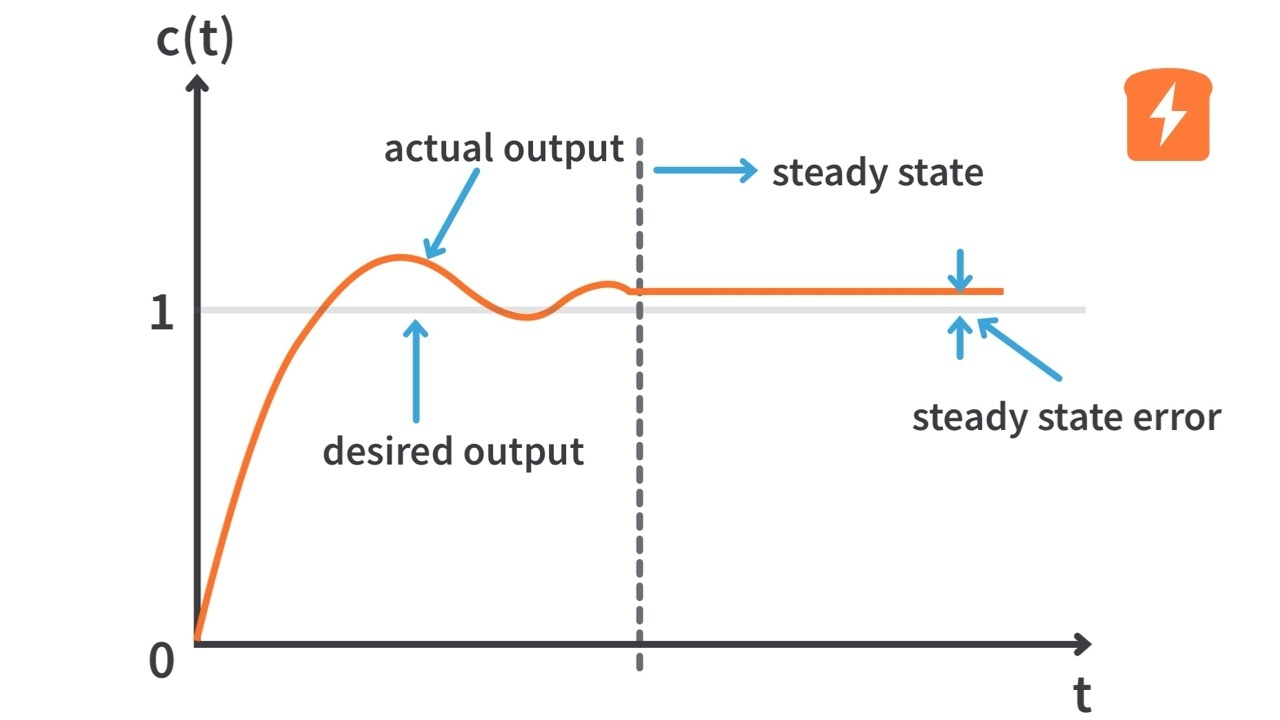
\includegraphics[width=190pt, height=110pt]{images/PID-I.png}
	\end{figure}
	\textbf{D – Derivative Control} จะคำนวณจากอัตราการเปลี่ยนแปลงของ Error เพื่อลดการ Overshoot และช่วยเพิ่มความเสถียร โดยมีสมการคือ $D_{\mathnormal{output}} = K_d \times \frac{de}{dt}$
	\begin{figure}[H]
	\centering
	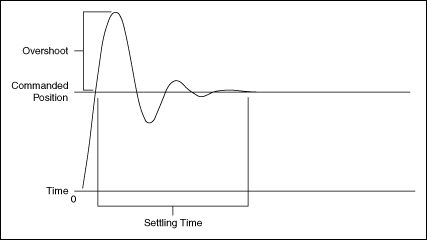
\includegraphics[width=190pt, height=110pt]{images/PID-D.png}
	\end{figure}
	จึงจะได้สมการรวมเป็น \vspace{0.2em}
		\[
			u(t) = \left( K_p \times e(t) \right) + \left(  K_i \times \int e(t) dt \right) + \left( K_d \times \frac{de}{dt} \right)
		\]
	\vspace{0.2em}
	\noindent เมื่อ $u(t)$ คือค่าคำสั่งที่ส่งไปควบคุมระบบ, $e(t)$ คือ Error ที่ขึ้นกับเวลา และ $K_p$, $K_i$, $K_d$ คือค่าคงที่ต้องทำการปรับจูน
\end{adjustwidth}

\subsection*{การทำงานของ Fast Fourier Transform (FFT)}
\begin{adjustwidth}{2em}{0em}
	\indent Fast Fourier Transform: FFT คือ Algorithm ที่นำ Fourier Series มาใช้เพื่อแปลงสมการหรือกราฟจาก Time Domain ไปเป็น Frequency Domain โดยเป็นวิธีที่พัฒนามาจาก Discrete Fourier Transform: DFT โดย \\[0.2em]
	\textbf{Continuous Fourier Transform} มีสมการคือ
	\[
		X(f) = \int_{-\infty}^{\infty} x(t) e^{-i \pi \xi x} dx
	\]
	และ \textbf{Discrete Fourier Transform} มีสมการดังนี้ 
	\begin{align*}
		X(k) &= \sum_{n = 0}^{N - 1} x(n) e^{-j 2 \pi \frac{k}{N} n} \\[0.5em]
		x(n) &= \frac{1}{N} \sum_{k = 0}^{N - 1} X(k) e^{+j 2 \pi \frac{k}{N} n}
	\end{align*}
\end{adjustwidth}

\subsection*{การทำงานหุ่นยนต์ (Workflow ของ PID line follower)}
Flow การทำงาน: Sensor $\rightarrow$ FFT filter $\rightarrow$ Line position $\rightarrow$ Error $\rightarrow$ PID $\rightarrow$ Motor Mix
\begin{adjustwidth}{2em}{0em}
	\begin{enumerate}
		\item Sensor: IR/Light Sensor/Color Sensor แล้วอ่านเป็น Vector $s_i$
		\item ตำแหน่งเส้น: ใช้ Weighted Average จะได้ $\displaystyle \mathit{pos} = \frac{\sum_{i} w_i s_i}{\sum_{i} s_i}$
	\end {enumerate}
\end{adjustwidth}

% \subsection*{การต่อวงจร}

\subsection*{ส่วนประกอบของหุ่นยนต์}
\begin{adjustwidth}{2em}{0em}
	\begin{enumerate}
		\item \textbf{Microcontroller - Arduino Nano ESP32} \\
			\indent ใช้ Chip NORA-W106-10B Module ตัวบอร์ดมีขนาด 17.78 x 40.64 mm มาพร้อมกับระบบ Wifi และ Bluetooth ใช้พลังงานต่ำ มีหน่วยความจำถาวรขนาด 16MB และหน่วยความจำ PSRAM อีก 8MB ประกอบด้วย Analog Pins จำนวน 8 Pin และ Digital Pins 14 Pin ใช้ในการรับและส่งข้อมูล พร้อมกับช่อง USB-C สำหรับจ่ายไฟ (ไม่เกิน 5V และจะถูกแปลงเป็น 3.3V เป็น Logic Power) ที้งนี้ บอร์ดจะใช้ Logic Power คือ 3.3V และอัปโหลดโปรแกรม (โดยการเขียนโปรแกรมสามารถเขียนผ่าน Arduino IDE) \\
			โดยในโครงงานนี้ใช้ในการเขียนโปรแกรมของฟังก์ชันที่เกี่ยวกับระบบเดินตามเส้นของหุ่นยนต์
		\item \textbf{Sensors}
			 \begin{itemize}
				\item \textbf{Sensor ตรวจจับเส้น} ชุดตรวจจับแสงสะท้อน ประกอบด้วยอินฟราเรด LED 8 คู่ และ phototransistor 8 ตัว เพื่อวัดค่าแสงสะท้อนจากพื้นผิว Sensor แต่ละตัวจะปล่อยแสงอินฟราเรดออกไป เมื่อแสงกระทบกับพื้นผิวจะสะท้อนกลับมายัง phototransistor และ เนื่องจากพื้นผิวที่มีสีเข้มจะดูดซับแสงมากกว่าพื้นผิวที่มีสีอ่อน ทำให้ sensor สามารถแยกแยะความแตกต่างของพื้นผิวได้ และสามารถต่อเข้ากับ Arduino nano esp32 ได้โดยใช้สาย jumper
				\item \textbf{Gyro Sensor - BNO085 9DOF Orientation IMU} คือเซนเซอร์วัดการเคลื่อนไหวแบบ 9 แกนที่รวม Accelerometer Gyroscope และ Magnetometer ที่ทำหน้าที่วัดความเร่ง การหมุน และทิศทางของสนามแม่เหล็กตามลำดับ ทำให้สามารถระบุทิศทาง การเอียง และการเคลื่อนไหวของอุปกรณ์ได้
			\end{itemize}
		\item \textbf{Motors - N20 Micrometal Gear Motor} \\
			\indent มอเตอร์ DC เกียร์โลหะขนาดเล็ก (Micro Metal Gearmotor) ใช้แปรงถ่านแบบ HPCB (High-Performance Carbon Brush) ซึ่งทนกระแสและความร้อนได้ดีกว่าแบบทั่วไป ตัวเรือนและชุดเกียร์ทำจาก โลหะ แข็งแรง ขนาดมาตรฐานตระกูล N20 หน้าตัดประมาณ 10 × 12 มม. ความยาวรวมเกียร์ราว 26–30 มม. ใช้แรงดันไฟ 6V DC ความเร็วรอบเอาต์พุตขึ้นกับอัตราทด (1:20 1750 RPM) ให้แรงบิดสูงเมื่อเทียบกับขนาด ระบบไฟฟ้าเป็น DC ธรรมดา กลไกการทำงาน คือมอเตอร์หมุนรอบสูงแล้วส่งกำลังผ่านชุดเกียร์โลหะเพื่อลดรอบและเพิ่มแรงบิด การเชื่อมต่อ เป็นมอเตอร์ 2 สาย ต้องต่อผ่านไดรเวอร์มอเตอร์ (เช่น TB6612FNG) โดยต่อสายมอเตอร์เข้าขา A01/A02 หรือ B01/B02, ต่อไฟ VM = 6V, VCC = 3.3V หรือ 5V, และ GND ร่วมกัน ควบคุมทิศทางด้วยขา IN1/IN2 และควบคุมความเร็วด้วย PWM ไม่ควรต่อเข้าขาไมโครคอนโทรลเลอร์โดยตรง การใช้งาน เหมาะกับรถหุ่นยนต์ขนาดเล็ก line follower, mini rover, กลไกขับเคลื่อนน้ำหนักเบา และงาน STEM/Arduino ที่ต้องการความทนทาน ขนาดเล็ก และควบคุมความเร็วได้แม่นยำ
		\item \textbf{Motor Driver - TB6612FNG Dual Motor Driver Carrier} \\
			เป็นบอร์ดไดรเวอร์มอเตอร์แบบคู่ ขนาดเล็กประมาณ 21 × 20 มม. ใช้ระบบ H-Bridge 2 ช่อง สำหรับควบคุมมอเตอร์ DC ได้ 2 ตัวหรือสเต็ปเปอร์ 1 ตัว รองรับแรงดันมอเตอร์ VM ~4.5–13.5V, แรงดันลอจิก VCC 2.7–5.5V (ใช้กับ Arduino/ESP32/MCU 3.3–5V ได้), กระแส 1A ต่อช่อง (Peak ~3A ชั่วคราว) มีระบบป้องกันความร้อนและ standby | ขา (Pin) หลักได้แก่ VM, VCC, GND, A01/A02 (Motor A), B01/B02 (Motor B), AIN1/AIN2, BIN1/BIN2 (กำหนดทิศทาง), PWMA/PWMB (PWM คุมความเร็ว), STBY (ต้อง HIGH เพื่อเปิดใช้งาน) การเชื่อมต่อ คือ ต่อมอเตอร์เข้าขา A/B, ต่อ VM เข้ากับแบต/ไฟมอเตอร์, VCC เข้ากับไฟลอจิก MCU และ GND ร่วมกัน, ต่อขาควบคุมเข้าขา Digital/PWM ของ MCU | การจ่ายไฟ แยกไฟมอเตอร์กับไฟลอจิกได้แต่ต้องกราวด์ร่วม | โปรแกรม ใช้สั่งทิศทางด้วย IN1/IN2 และปรับความเร็วด้วย PWM (เช่น analogWrite) พร้อมดึง STBY เป็น HIGH | การใช้งาน เหมาะกับรถหุ่นยนต์ รถบังคับ สายพาน กลไกขนาดเล็ก ที่ต้องการควบคุมความเร็วและทิศทางอย่างมีประสิทธิภาพและประหยัดพลังงานกว่า L298N
		\item \textbf{ล้อรถ}
			\begin{itemize}
				\item \textbf{ล้อหน้า} Pololu Ball Caster มีขนาดความสูง 0.4 นิ้วและสามารถเพิ่มความสูงได้ถึง 0.6 นิ้วด้วย Spacer เป็นล้อที่ถูกออกแบบเพื่อหุ่นยนต์ขนาดเล็กสามารถรับน้ำหนักได้ไม่มากโดยล้อนี้สามารถถอดแยกประกอบชิ้นส่วนได้ง่าย ๆ
				\item \textbf{ล้อหลัง} Pololu 40 mm Wheels มีขนาดกะทัดรัด น้ำหนักเบา ติดตั้งง่าย ล้อมีเส้นผ่าศูนย์กลาง 40mm ด้านนอกหุ้มด้วยยางซิลิโคน ซึ่งให้แรงเสียดทานสูงกว่ายางธรรมดา ทำให้ล้อเกาะพื้นได้ดี ไม่ลื่นง่าย เหมาทั้งพื้นเรียบและไม่เรียบ
			\end{itemize}
		\item \textbf{โครงรถ}
			ออกแบบเป็นโมเดลสามมิติและปริ๊นโดย 3D Printer โดยใช้วัสดุเป็น PLA
		\item \textbf{แบตเตอรี่ - LiPo Battery} \\
			เป็นแบตเตอรี่ Lithium Polymer ประเภทหนึ่งที่ใช้ Polymer Electrolyes ซึ่งต่างจากแบบทั่วไปที่ใช้สารละลาย Electrolytes ขนาดความจุ 850mAh ค่าอัตราการจ่ายไฟ 75C จำนวน 2 เซลล์
		\item \textbf{สายไฟ - สาย Jumper} \\
			ใช้เป็นสายเชื่อมระหว่างอุปกรณ์ต่างๆ มีปลายสาย 2 แบบคือตัวผู้และตัวเมียโดยออกแบบให้ตัวผู้และตัวเมียสามารถต่อเชื่อมกันได้เลยโดยไม่ต้องบัดกรีเป็นการเพิ่มความสะดวกสบาย แต่อาจมีบางจุดที่อุปกรณ์ไม่มีขาหรือช่องให้เชื่อมอาจมีความจำเป็นต้องบัดกรี
		\item \textbf{DC - DC Multi Output Buck Converter} \\
			คือวงจรแปลงแรงดันไฟฟ้ากระแสตรงแบบ Step-Down (Buck) ที่รับไฟ DC แรงดันสูงกว่าหนึ่งค่า แล้วแปลงออกมาเป็น หลายแรงดันพร้อมกัน เช่น 12V $\rightarrow$ 5V, 3.3V และ 1.8V ในบอร์ดเดียว ใช้หลักการสวิตชิ่งความถี่สูงร่วมกับ ตัวเหนี่ยวนำ (inductor), ไดโอดหรือ synchronous MOSFET, คาปาซิเตอร์ และตัวควบคุม PWM เพื่อให้ได้ประสิทธิภาพสูง (มัก 80–95\%) และสูญเสียความร้อนต่ำ เหมาะกับระบบที่มีหลายภาคจ่ายไฟ เช่น หุ่นยนต์, บอร์ดไมโครคอนโทรลเลอร์, SBC, ระบบ IoT หรืออุปกรณ์พกพา สเปกสำคัญ ที่ควรดูคือแรงดันอินพุตที่รองรับ, ค่าแรงดันเอาต์พุตแต่ละช่อง, กระแสสูงสุดต่อช่อง, ripple noise, ประสิทธิภาพ, ความถี่สวิตชิ่ง และระบบป้องกันเช่น OCP (กันกระแสเกิน), OVP (กันแรงดันเกิน), OTP (กันร้อนเกิน) การเชื่อมต่อ คือจ่ายไฟ DC เข้าขา VIN และ GND แล้วรับไฟออกจากขา VOUT แต่ละแรงดันพร้อมกราวด์ร่วม บางรุ่นปรับแรงดันได้ผ่านโพเทนชิโอมิเตอร์หรือขา feedback การใช้งาน ช่วยลดจำนวนโมดูลแปลงไฟหลายตัวให้เหลือบอร์ดเดียว ประหยัดพื้นที่ ลดความซับซ้อนสายไฟ และเพิ่มเสถียรภาพของระบบจ่ายไฟรวม โดยต้องเลือกให้กระแสรวมโหลดไม่เกินพิกัดของแต่ละเอาต์พุตและมีการระบายความร้อนเหมาะสม
				\begin{figure}[H]
					\centering
					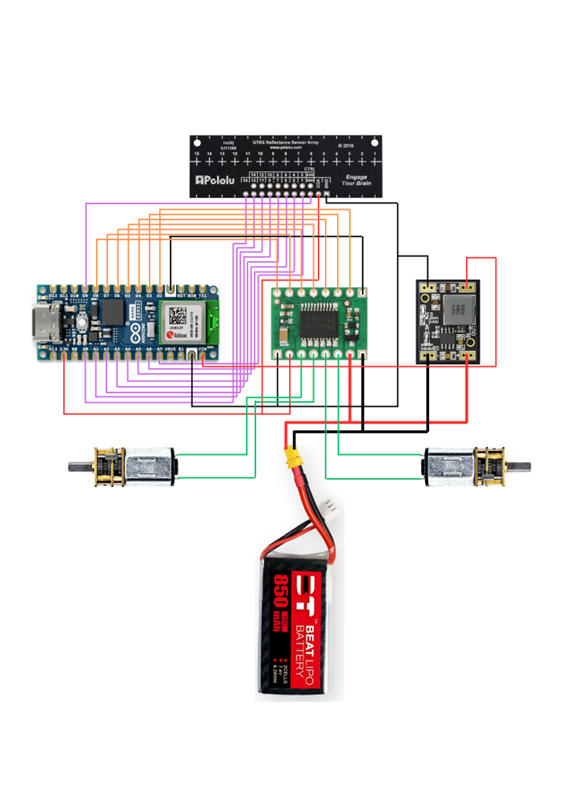
\includegraphics[width=240pt, height=340pt]{images/WiringDiagram.png}
				\end{figure}
	\end{enumerate}
\end{adjustwidth}

\subsection*{โครงงาน/งานวิจัยที่เกี่ยวข้อง} \vspace{-1em}
\begin{adjustwidth}{4em}{0em}
	\subsubsection*{เกี่ยวกับระบบ PID} \vspace{-0.75em}
	\noindent \textbf{[1] Chen et al., 2010 — Self-Tuning PID จากคุณลักษณะความถี่} \\
		\indent แนวคิด: ใช้ Frequency Domain เพื่อปรับ $K_p$, $K_i$, $K_d$ โดยอัตโนมัติทำการเก็บสัญญาณ Error เป็นช่วง ๆ แล้วทำ FFT เพื่อดู Oscillation Peak แล้ว ปรับ $K_d $ เพื่อลด Oscillation แล้วจูน $K_p$      และ $K_i$ \\
	\textbf{[6] Benrabah et al., 2021 — AFSNNPID (Adaptive Fourier-Series Neural-Network PID)} \\
		\indent แนวคิด: ใช้โครงข่าย FSNN (ฐาน $\sin$/$\cos$) ปรับ $K_p$, $K_i$, $K_d$ ด้วย delta-rule แล้ววิเคราะห์เสถียรภาพด้วย small-gain theorem; ซึ่งเหมาะงานเรียลไทม์เพราะคำนวณได้รวดเร็ว \\
	\textbf{[7] Ringwood \& O’Dwyer, 1994 — Frequency Domain Based Self-Tuning PID} \\
		\indent แนวคิด: จะปรับจูนด้วยการประเมินคุณสมบัติความถี่ของระบบระหว่างทำงาน แล้วปรับ PID Parameters ให้สามารถเดินตามเส้นได้อย่างรวดเร็วมี ประสิทธิภาพและแม่นยำ

	\subsubsection*{เกี่ยวกับหุ่นยนต์เดินตามเส้น} \vspace{-0.75em}
	\textbf{Mehran pakdaman, M. Mehdi Sanaatiyan, Mahdi Rezaei Ghahroudi, 2010 — A Line Follower Robot from design to Implementation: Technical issues and problems} \\
	\indent ทำงานเกี่ยวกับการสร้างหุ่นยนต์เดินตามเส้นแบบทั่วไป (น้ำหนัก 300 กรัม) โดยประกอบเซ็นเซอร์เดี่ยวหลายๆคู่เข้าด้วยกันอ่านเป็นค่า Analog และ แปลงเป็นดิจิทัล (digital) และ จึงส่งข้อมูลไปให้ AVR Microcontroller MEGA 16 (เขียนด้วยภาษา C และส่งโปรแกรมหลัง Compilation ผ่าน Programmer) และ ส่งข้อมูลไปให้ Driver IC L298 ที่ทำการควบคุมมอเตอร์ต่อ โดยมีรายละเอียดโดยสรุปดังนี้: 
	\vspace{-0.5em}
	\begin{enumerate}
		\item เซ็นเซอร์ต้องมีการครอบไม่ให้แสงจากภายนอกเข้าสู่ระบบและเซ็นเซอร์มีระยะห่างจากพื้นผิว 0.2 ถึง 1 เซนติเมตร 
		\item ระยะห่างระหว่างเซ็นเซอร์จะแปรผันโดยตรงกับความหนาเส้นเดิน มิฉะนั้นหุ่นยนต์อาจไม่สามารถหมุนเลี้ยวได้ได้ทันเวลาเมื่อเข้าโค้ง 
		\item สำหรับหุ่นยนต์เดินตามเส้นขนาดเล็กที่มีเซ็นเซอร์จำนวนสองถึงสามอันสามารถใช้ประตูสัญญาณ”และ/หรือ”ได้แต่จะได้ผลลัพธ์ไม่แม่นยำและความเร็วตำ่รวมถึงไม่สามารถเลี้ยวผ่านทางโค้งยากๆได้ 
		\item มีการใช้มอเตอร์สองจังหวะแต่มีปัญหาได้แก่ ต้องป้อนข้อมูลสี่ข้อมูล, ต้องการ Driver จำนวนสองตัวเพื่อที่จะจ่ายไฟให้พอ ทำให้ยากต่อการใช้งานจึงแนะนำให้ใช้มอเตอร์เกียร์ (Gearbox Motor) เพราะมีเกียรและเพลาให้
		\item วัสดุแนะนำให้ใช้อลูมิเนียมเพราะมีนำ้หนักเบาและแข็งแรง 
		\item รูปร่างภายนอกไม่สำคัญ (ฟังก์ชันการทำงานสำคัญที่สุด) 
		\item ไม่แนะนำให้ใช้กาวทุกชนิดในการติดส่วนประกอบต่างแนะนำให้ใช้สกรู
	\end{enumerate}
	\vspace{-0.5em}
	\textbf{Theunis R. Botha* and P. Schalk Els, 2019 — Vehicle centre of mass, roll-centre and pitch-centre height estimation} \\
	\indent
	งานวิจัยด้านพารามิเตอร์นี้ชี้ให้เห็นว่า ตำแหน่งจุดศูนย์ถ่วงและความสูง roll/pitch center มีผลอย่างมากต่อการถ่ายน้ำหนักและความเสถียรในการเคลื่อนที่ขณะเลี้ยวหรือเร่งความเร็ว งานวิจัยนี้สามารถประยุกต์ใช้กับหุ่นยนต์เดินตามเส้นได้โดยตรง เนื่องจากถ้าหุ่นยนต์มีจุดศูนย์ถ่วงสูงเกินไปหรือการกระจายน้ำหนักไม่สมดุล จะทำให้การตอบสนองต่อคำสั่งPIDได้ไม่ดี ส่งผลให้เกิดการส่ายหรือหลุุดเส้่นหุ่นยนต์เดินตามเส้นที่ใช้นี้เป็นหุ่นยนต์เดินตามเส้นแบบขับเคลื่อนด้วย2ล้อโดยมีล้อขับเคลื่อนจำนวน2ล้อและล้อพยุงจำนวน1ล้อ โครงสร้างดังกล่าวช่วยให้สามารถปรับทิศทางการเคลือนที่ได้ด้วยการปรับล้อซ้ายและล้อขวา รวมถึงยังช่วยลดความซับซ้อนของการออกแบบโปรแกรม ตัวอย่างโครงสร้างทางกายภาพของหุ่นยนต์ได้แก่ ระยะห่างระหว่างฐานล้อซึ่งคือล้อซ้ายและล้อขวา เส้นผ้าศุนย์กลางของล้อขับเคลื่อนและล้อพยุง  โดยให้จุดศูนย์ถ่วงของรถโดยจัดให้อยู่ต่ำและอยู่บริเวณกึ่งกลางของล้อทั้งสอง โครงสร้างทางกายภาพเหล่านี้มีผลต่อการเลี้ยวและการควบคุมของรถ เพื่อเพิ่มความเสถียรในการเคลื่อนที่และลดการสั่นตัวของรถ \\
	\textbf{Line Follower Robot with PID Control} \\
	\indent
	งานวิจัยนี้มีจุดมุ่งหมายเพื่อออกแบบและสร้างหุ่นยนต์ติดตามเส้นโดยใช้อัลกอริธึมควบคุมแบบ Proportional-Integral-Derivative: PID และโค้ดภาษาซีระดับรีจิสเตอร์ ความก้าวหน้าในการนำทางอัตโนมัตินี้ช่วยแก้ปัญหาความท้าทายในการนำทางหุ่นยนต์เคลื่อนที่ไปตามเส้นทางที่กำหนดไว้ล่วงหน้าในสภาพแวดล้อมที่ควบคุมได้ โดยใช้เครื่องหมายและเซ็นเซอร์ที่สามารถระบุได้ เช่น เซ็นเซอร์ Hall-Effect และ Photo-Interrupter โครงการนี้ปรับปรุงวิธีการติดตามเส้นแบบดั้งเดิมโดยใช้การควบคุม PID ซึ่งปรับแต่งการตอบสนองของมอเตอร์เพื่อการนำทางที่ราบรื่นและแม่นยำยิ่งขึ้น โดยใช้ระบบควบคุมแบบวงปิดเพื่อลดข้อผิดพลาดผ่านการปรับเปลี่ยนตามตำแหน่งของหุ่นยนต์เทียบกับเส้น การนำตัวควบคุม PID มาใช้ในหุ่นยนต์ติดตามเส้นเพื่อเพิ่มความแม่นยำและความเร็วในการนำทาง โดยอธิบายว่าค่าเกนแบบสัดส่วนช่วยปรับปรุงการตอบสนองต่อการรบกวน แต่หากตั้งค่าสูงเกินไปอาจทำให้เกิดความไม่เสถียรได้ การควบคุมแบบอินทิกรัลช่วยขจัดข้อผิดพลาดในสภาวะคงที่ ในขณะที่การควบคุมแบบอนุพันธ์ช่วยลดการโอเวอร์ชูตและคาดการณ์ข้อผิดพลาดในอนาคต อย่างไรก็ตาม การควบคุมแบบอนุพันธ์อาจทำให้เกิดความไม่เสถียรเนื่องจากการขยายสัญญาณรบกวน งานวิจัยนี้มีจุดมุ่งหมายเพื่อเพิ่มประสิทธิภาพความสามารถของหุ่นยนต์ในการเคลื่อนที่ไปตามเส้นทางได้อย่างรวดเร็วและแม่นยำ โดยใช้ Microcontroller ที่เขียนโปรแกรมด้วยภาษา ARM C และใช้ข้อมูลจากอาร์เรย์เซ็นเซอร์สะท้อนแสงเพื่อคำนวณข้อผิดพลาดและปรับพารามิเตอร์ PID อย่างมีประสิทธิภาพ
\end{adjustwidth}

\section*{วิธีดำเนินงาน}
\textbf{กระบวนการออกแบบเชิงวิศวกรรม}
\begin{enumerate}
	\item \textbf{ระบุปัญหา}
	\begin{enumerate}
		\item 5W1H \\
			\begin{table}[H]
			\centering
			\renewcommand{\arraystretch}{1.35}
			\setlength{\tabcolsep}{8pt}

			\begin{tabular}{>{\centering\arraybackslash}p{5cm} p{10cm}}
			\hline
			\centering\textbf{คำถาม 5W1H} & 
			\centering\textbf{คำตอบ} \tabularnewline
			\hline

			ปัญหาหรือความต้องการเกิดขึ้นกับใคร (Who) &
			ผู้ที่ต้องการใช้เทคโนโลยีหุ่นยนต์เดินตามเส้นมาประยุกต์ใช้ในชีวิตประจำวัน
			\\ \hline

			ปัญหาหรือความต้องการคืออะไร (What) &
			การใช้เทคโนโลยีหุ่นยนต์เดินตามเส้นมาประยุกต์ใช้ในชีวิตประจำวัน
			\\ \hline

			ปัญหาหรือความต้องการเกิดขึ้นที่ใด (Where) &
			ใช้งานในพื้นที่ที่มีเส้นทางชัดเจนสำหรับหุ่นยนต์หรือพื้นที่ที่มีความอันตราย เช่น  
			ในโรงงานอุตสาหกรรม สถานที่ที่มีอันตรายสูง
			\\ \hline

			ปัญหาหรือความต้องการเกิดขึ้นเมื่อใด (Where) &
			เมื่อต้องใช้งานซ้ำในเส้นทางเดิม ต้องการลดต้นทุน ลดความผิดพลาด เมื่องานต้องอาศัยความแม่นยำสูง หรือในสถานการณ์ที่มีความเสี่ยง
			\\ \hline

			ทำไมจึงเกิดปัญหาหรือความต้องการนี้ (Why) &
			การขาดประสิทธิภาพและความปลอดภัยของมนุษย์ จึงต้องใช้หุ่นยนต์เดินตามเส้นช่วยในงานที่ต้องการความปลอดภัยและความสม่ำเสมอ
			\\ \hline

			ปัญหาหรือความต้องการมีลักษณะอย่างไร (How) &
			ต้องการระบบอัตโนมัติที่มีความแม่นยำและเชื่อถือได้ สามารถช่วยงานในพื้นที่อันตรายหรือซ้ำซ้อนได้
			\\ \hline
			\end{tabular}
			\end{table}
		\item แผนผังก้างปลา (Fishbone Diagram)
			\begin{figure}[H]
				\centering
				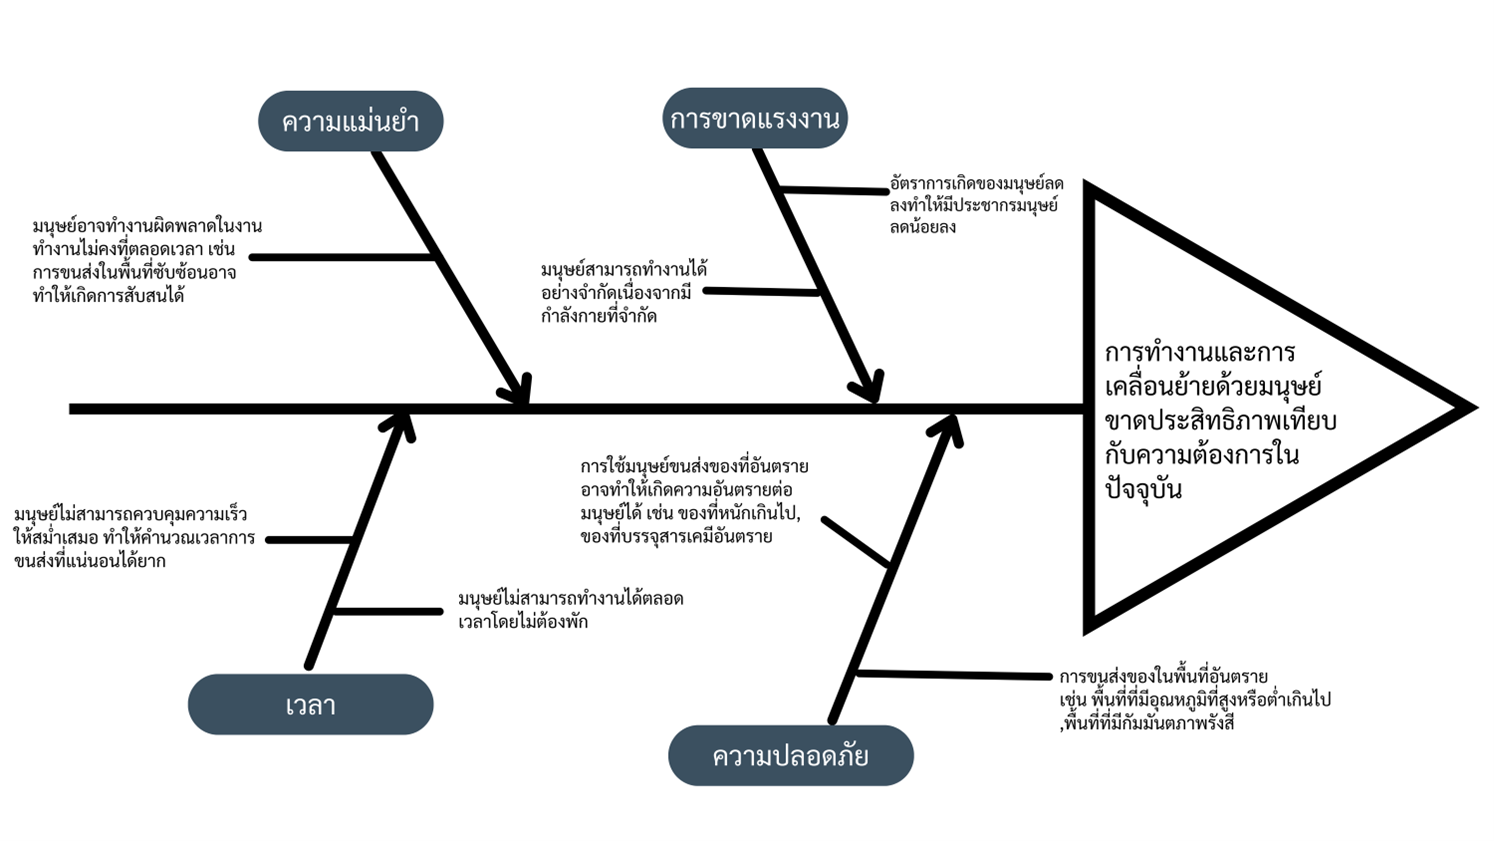
\includegraphics[width=360pt, height=202pt]{images/FishboneDiagram.png}
			\end{figure}
	\end{enumerate}
	\item \textbf{รวมรวมข้อมูลและแนวคิดที่เกี่ยวกับปัญหา}
	\begin{enumerate}
		\item ส่วนประกอบของหุ่นยนต์
		\begin{itemize}
			\item Microcontroller: Arduino Nano ESP32
			\item Sensor: QTRX-MD-08A Reflectance Sensor Array
			\item Motors: 6V HPCB Micro Metal Gear Motor
			\item Motor driver: TB6612FNG Dual Motor Driver Carrier
			\item แบตเตอรี่ LIPO BATTERY
			\item ล้อรถ Pololu ball caster และ Pololu 40mm wheels
			\item โครงรถ
			\item สายไฟ: สาย Jumper
			\item Converter: dc-dc multi-output buck converter
		\end{itemize}
		\item การทำงานของระบบต่าง ๆ
		\begin{itemize}
			\item ทฤษฏีการทำงานของระบบPID
			\item ทฤษฎีการทำงานของ Fast Fourier Transform (FFT)
			\item การทำงานหุ่นยนต์ (Workflow ของ PID line follower)
			\item การต่อวงจร
		\end{itemize}
		\item โครงงาน/งานวิจัยที่เกี่ยวข้อง \\
		โครงงาน/งานวิจัยเกี่ยวกับระบบ PID
		\begin{itemize}
			\item Chen et al., 2010 — Self-Tuning PID จากคุณลักษณะความถี่
			\item Benrabah et al., 2021 — AFSNNPID (Adaptive Fourier-Series Neural-Network PID)
			\item Ringwood \& O’Dwyer, 1994 — Frequency Domain Based Self-Tuning PID
		\end{itemize}
		โครงงาน/งานวิจัยเกี่ยวกับหุ่นยนต์เดินตามเส้น
		\begin{itemize}
			\item Mehran pakdaman, M. Mehdi Sanaatiyan, Mahdi Rezaei Ghahroudi, 2010 — A Line Follower Robot from design to Implementation: Technical issues and problems
			\item Theunis R. Botha* and P. Schalk Els, 2019 — Vehicle centre of mass, roll-centre and pitch-centre height estimation
			\item Onur Erbay, Abdullah Burhan Doğan, Enes Devecioğlu, 2024 — Line Follower Robot with PID Control
		\end{itemize}
		\item Component Option Table
			\begin{table}[H]
			\centering
			\renewcommand{\arraystretch}{1.35}

			% Make long text wrap
			\begin{tabular}{|p{1cm}|p{2cm}|p{1.75cm}|p{5cm}|p{5cm}|}
			\hline

			\multicolumn{3}{|c|}{\textbf{Light Reflectance Sensor}} 
			& \textbf{แบบที่ 1 QTRX-MD-08A} 
			& \textbf{แบบที่ 2 SunFounder I2C 5-Channel Module} 
			\\ \hline

			\multicolumn{3}{|c|}{\textbf{ข้อมูลรายละเอียด}} 
			& \multicolumn{1}{p{5cm}|}{
			QTRX-MD-08A Reflectance Sensor Array เป็น เซนเซอร์ตรวจจับแสงแบบ Array 8 ช่อง ภายในประกอบด้วย IR LED และ Phototransistor จำนวน 8 คู่ ออกแบบมาเพื่อใช้ตรวจจับความแตกต่างของการสะท้อนแสงระหว่างเส้นสีดำและพื้นสีอ่อนรองรับแรงดันไฟฟ้า 3.3–5.0V ให้เอาต์พุตแบบ Analog สามารถอ่านค่าได้โดยตรงผ่านขา ADC ของไมโครคอนโทรลเลอร์ ใช้กระแสไฟฟ้าโดยประมาณ 80–100 mA เมื่อเปิดใช้งาน IR LED ครบทุกช่อง มีระยะการตรวจจับที่เหมาะ สามารถให้ข้อมูลต่อเนื่องและละเอียด ทำให้รองรับการควบคุมแบบ PID Control ได้ดี โดยเฉพาะการวิ่งตามเส้นโค้งหรือเส้นที่มีความซับซ้อน
			} 
			& \multicolumn{1}{p{5cm}|}{
			SunFounder I2C 5-Channel Line Follower Module เป็นโมดูลตรวจเส้นแบบ 5 ช่อง ใช้เซนเซอร์ TCRT5000 พร้อมไมโครคอนโทรลเลอร์บนบอร์ดใช้ แรงดันไฟ 5V และสื่อสารกับ Arduino ผ่าน I2C (4 ขา) ให้เอาต์พุตแบบ Digital ประหยัดพอร์ต Arduino และอ่านค่าสัญญาณได้ง่ายกว่าแบบ digital ปกติ ใช้กระแสไฟฟ้าโดยประมาณ 20–40 mA ขณะทำงาน มีปุ่ม RESET และ โพเทนชิโอมิเตอร์ สำหรับปรับความไวของเซนเซอร์ตามพื้นผิวที่ต่างกัน เหมาะสำหรับใช้งานพื้นฐาน
			}
			\\ \hline

			\multirow{5}{*}{\rotatebox{90}{\parbox{3cm}{\centering\textbf{เกณฑ์การพิจารณา}}}}
			& ปริมาณกระแสไฟฟ้าที่ใช้ & น้อย = 1 มาก = 0
			& 0 & 1 \\ \cline{2-5}

			& จำนวนเซนเซอร์ & มาก = 1 น้อย = 0
			& 1 & 0 \\ \cline{2-5}

			& ความละเอียดข้อมูลที่ได้ & มาก = 2 กลาง = 1 น้อย = 0
			& 2 & 1 \\ \cline{2-5}

			& ความเสถียรเมื่อมีแสงรบกวน & มาก = 2 กลาง = 1 น้อย = 0
			& 2 & 1 \\ \cline{2-5}

			& ราคา & น้อย  = 2 กลาง = 1 มาก = 0
			& 1 & 2 \\ \hline

			\multicolumn{3}{|c|}{\textbf{ผลรวม}} & \textbf{6} & \textbf{5} \\ \hline

			\end{tabular}
			\end{table}
			\begin{table}[H]
			\centering
			\renewcommand{\arraystretch}{1.35}

			% Make long text wrap
			\begin{tabular}{|p{1cm}|p{2cm}|p{1.75cm}|p{5cm}|p{5cm}|}
			\hline

			\multicolumn{3}{|c|}{\textbf{Microcontroller}} 
			& \textbf{แบบที่1 Arduino UNO R4} 
			& \textbf{แบบที่2 Arduino NANO ESP32} 
			\\ \hline

			\multicolumn{3}{|c|}{\textbf{ข้อมูลรายละเอียด}} 
			& \multicolumn{1}{p{5cm}|}{
			Arduino UNO R4 เป็นบอร์ดไมโครคอนโทรลเลอร์มาตรฐานของ Arduino เหมาะสำหรับงานควบคุมพื้นฐานและการเรียนรู้ มีความเสถียรในการทำงานและรองรับการใช้งานทั่วไปได้ดีทำงานที่แรงดันไฟฟ้า 5V มีขา Digital และ Analog I/O สำหรับเชื่อมต่อเซนเซอร์และอุปกรณ์ต่างๆ ได้หลากหลายโดยมี Analog 6 pin และ Digital 16 pinปริมาณกระแสไฟฟ้าที่ใช้ โดยประมาณอยู่ที่ 40–70 mA ซึ่งค่อนข้างสูงกว่าไมโครคอนโทรลเลอร์ขนาดเล็ก ทำให้เหมาะกับการใช้งานที่มีแหล่งจ่ายไฟเพียงพอมีขนาดค่อนข้างใหญ่เมื่อเทียบกับบอร์ดแบบอื่น
			} 
			& \multicolumn{1}{p{5cm}|}{
			Arduino NANO ESP32
เป็นบอร์ดไมโครคอนโทรลเลอร์ขนาดเล็กที่ใช้ชิป ESP32
มีประสิทธิภาพการประมวลผลสูง 
ทำงานที่แรงดันไฟฟ้า 3.3V รองรับการเชื่อมต่อกับเซนเซอร์หลายชนิด และสามารถอ่านค่า Analog และ Digital ได้โดยมี Analog 8 pin และ Digital 14 pin
ปริมาณกระแสไฟฟ้าที่ใช้ โดยประมาณอยู่ที่ 20–50 mA ในโหมดทำงานปกติ และอาจเพิ่มขึ้นเป็น 100–200 mA ขณะใช้งาน 
Wi-Fi หรือ Bluetooth ซึ่งยังถือว่าประหยัดพื้นที่และให้ประสิทธิภาพสูง
มีระบบสื่อสารไร้สายในตัว มีขนาดเล็ก กะทัดรัด  และสามารถใช้งานร่วมกับระบบควบคุม 
เช่น PID Control ได้อย่างมีประสิทธิภาพ
เหมาะแก่การใช้งานบน
เบรดบอร์ด


			}
			\\ \hline

			\multirow{5}{*}{\rotatebox{90}{\parbox{3cm}{\centering\textbf{เกณฑ์การพิจารณา}}}}
			& ประสิทธิ
ภาพการประมวลผล
 & สูง = 1 ต่ำ = 0
			& 0 & 1 \\ \cline{2-5}

			& ขนาดและความกะทัดรัด & เล็ก = 1 ใหญ่ = 0
			& 0 & 1 \\ \cline{2-5}

			& รูปแบบการเชื่อมต่อ & มาก = 1 น้อย = 0
			& 0 & 1 \\ \cline{2-5}

			& หน่วยความจำ & มาก = 2 กลาง = 1 น้อย = 0
			& 1 & 2 \\ \cline{2-5}

			& ราคา & ต่ำ = 1 สูง = 0
			& 1 & 0 \\ \hline

			\multicolumn{3}{|c|}{\textbf{ผลรวม}} & \textbf{2} & \textbf{5} \\ \hline

			\end{tabular}
			\end{table}
			\begin{table}[H]
			\centering
			\renewcommand{\arraystretch}{1.35}

			% Make long text wrap
			\begin{tabular}{|p{1cm}|p{2cm}|p{1.75cm}|p{5cm}|p{5cm}|}
			\hline

			\multicolumn{3}{|c|}{\textbf{Motor Driver}} 
			& \textbf{แบบที่1 TB6612FNG Dual Motor Driver Carrier } 
			& \textbf{แบบที่2 L298N Motor Driver Board Module} 
			\\ \hline

			\multicolumn{3}{|c|}{\textbf{ข้อมูลรายละเอียด}} 
			& \multicolumn{1}{p{5cm}|}{
			TB6612FNG Dual Motor Driver Carrier เป็นโมดูลไดรเวอร์มอเตอร์แบบ Dual H-Bridge ที่ใช้ชิป TB6612FNG เหมาะสำหรับงานควบคุมมอเตอร์ DC และมอเตอร์เกียร์ขนาดเล็ก รวมถึงงานหุ่นยนต์และการเรียนรู้ด้านระบบควบคุม มีความเสถียรและใช้งานร่วมกับไมโครคอนโทรลเลอร์ได้หลากหลาย เช่น Arduino
ทำงานที่แรงดันไฟฟ้าฝั่งลอจิก 2.7–5.5V และแรงดันไฟฟ้าสำหรับมอเตอร์ 4.5–13.5V รองรับการควบคุมทิศทางและความเร็วของมอเตอร์ผ่านสัญญาณ Digital และ PWM ได้อย่างแม่นยำ
สามารถจ่ายกระแสให้มอเตอร์ได้สูงสุดประมาณ 1.2A ต่อช่อง และสูงสุด 3.2A แบบชั่วขณะ เหมาะสำหรับมอเตอร์ขนาดเล็กถึงขนาดกลาง โดยมีระบบป้องกันความร้อนและการลัดวงจรภายใน
มีขนาดกะทัดรัด น้ำหนักเบา เหมาะสำหรับติดตั้งบนเบรดบอร์ด ช่วยลดภาระของไมโครคอนโทรลเลอร์ในการขับมอเตอร์โดยตรง และเพิ่มความปลอดภัยในการใช้งาน

			} 
			& \multicolumn{1}{p{5cm}|}{
ข้อมูล
รายละเอียด
 	TB6612FNG Dual Motor Driver Carrier เป็นโมดูลไดรเวอร์มอเตอร์แบบ Dual H-Bridge ที่ใช้ชิป TB6612FNG เหมาะสำหรับงานควบคุมมอเตอร์ DC และมอเตอร์เกียร์ขนาดเล็ก รวมถึงงานหุ่นยนต์และการเรียนรู้ด้านระบบควบคุม มีความเสถียรและใช้งานร่วมกับไมโครคอนโทรลเลอร์ได้หลากหลาย เช่น Arduino
ทำงานที่แรงดันไฟฟ้าฝั่งลอจิก 2.7–5.5V และแรงดันไฟฟ้าสำหรับมอเตอร์ 4.5–13.5V รองรับการควบคุมทิศทางและความเร็วของมอเตอร์ผ่านสัญญาณ Digital และ PWM ได้อย่างแม่นยำ
สามารถจ่ายกระแสให้มอเตอร์ได้สูงสุดประมาณ 1.2A ต่อช่อง และสูงสุด 3.2A แบบชั่วขณะ เหมาะสำหรับมอเตอร์ขนาดเล็กถึงขนาดกลาง โดยมีระบบป้องกันความร้อนและการลัดวงจรภายใน
มีขนาดกะทัดรัด น้ำหนักเบา เหมาะสำหรับติดตั้งบนเบรดบอร์ด ช่วยลดภาระของไมโครคอนโทรลเลอร์ในการขับมอเตอร์โดยตรง และเพิ่มความปลอดภัยในการใช้งาน
	L298N Motor Driver Board Module เป็นโมดูลไดรเวอร์มอเตอร์แบบ Dual H-Bridge ที่ใช้ไอซี ชิป L298N เหมาะสำหรับงานควบคุมมอเตอร์ DC และ
สเต็ปเปอร์มอเตอร์ในงานพื้นฐาน เช่น รถหุ่นยนต์ ระบบทดลอง และการเรียนรู้ด้านการควบคุมมอเตอร์ สามารถใช้งานร่วมกับไมโครคอนโทรลเลอร์ได้หลากหลาย เช่น Arduino
ทำงานที่แรงดันไฟฟ้าสำหรับมอเตอร์อยู่ในช่วงประมาณ 5–35V และแรงดันไฟฟ้าฝั่งลอจิก 5V รองรับการควบคุมทิศทางการหมุนและความเร็วของมอเตอร์ผ่านขา Digital และสัญญาณ PWM
สามารถจ่ายกระแสให้มอเตอร์ได้สูงสุดประมาณ 2A ต่อช่อง (สูงสุดตามสเปกไอซี) เหมาะสำหรับมอเตอร์ DC ขนาดกลาง อย่างไรก็ตามมีการสูญเสียพลังงานค่อนข้างสูงและเกิดความร้อนมากเมื่อใช้งานต่อเนื่อง จึงมักมีฮีตซิงก์ติดตั้งมาบนบอร์ด
มีขนาดค่อนข้างใหญ่และแข็งแรง เหมาะสำหรับการทดลองบนโต๊ะหรือการติดตั้งแบบถาวร ไม่เหมาะกับงานที่ต้องการความกะทัดรัดหรือประสิทธิภาพพลังงานสูง แต่มีข้อดีคือราคาประหยัด หาได้ง่าย และใช้งานไม่ซับซ้อน
			}
			\\ \hline

			\multirow{5}{*}{\rotatebox{90}{\parbox{3cm}{\centering\textbf{เกณฑ์การพิจารณา}}}}
			& การใช้พลังงาน
 & ต่ำ = 1 สูง = 0
			& 1 & 2 \\ \cline{2-5}

			& ขนาด
และความกะทัดรัด
 & เล็ก = 1 ใหญ่ = 0
			& 1 & 0 \\ \cline{2-5}

			& กระแสขับมอเตอร์ต่อช่อง & มาก = 1 น้อย = 0
			& 0 & 1 \\ \cline{2-5}

			& การจัดการความร้อน & ดี=1
ไม่ดี=0
			& 1 & 0 \\ \cline{2-5}

			& ราคา & ต่ำ = 1 สูง = 0
			& 0 & 1 \\ \hline

			\multicolumn{3}{|c|}{\textbf{ผลรวม}} & \textbf{3} & \textbf{2} \\ \hline

			\end{tabular}
			\end{table}
		\end{enumerate}
	\item ออกแบบวิธีการแก้ปัญหา
	\begin{enumerate}
		\item ออกแบบโครงรถโดยการใช้ Function Analysis Diagram
			\begin{figure}[H]
				\centering
				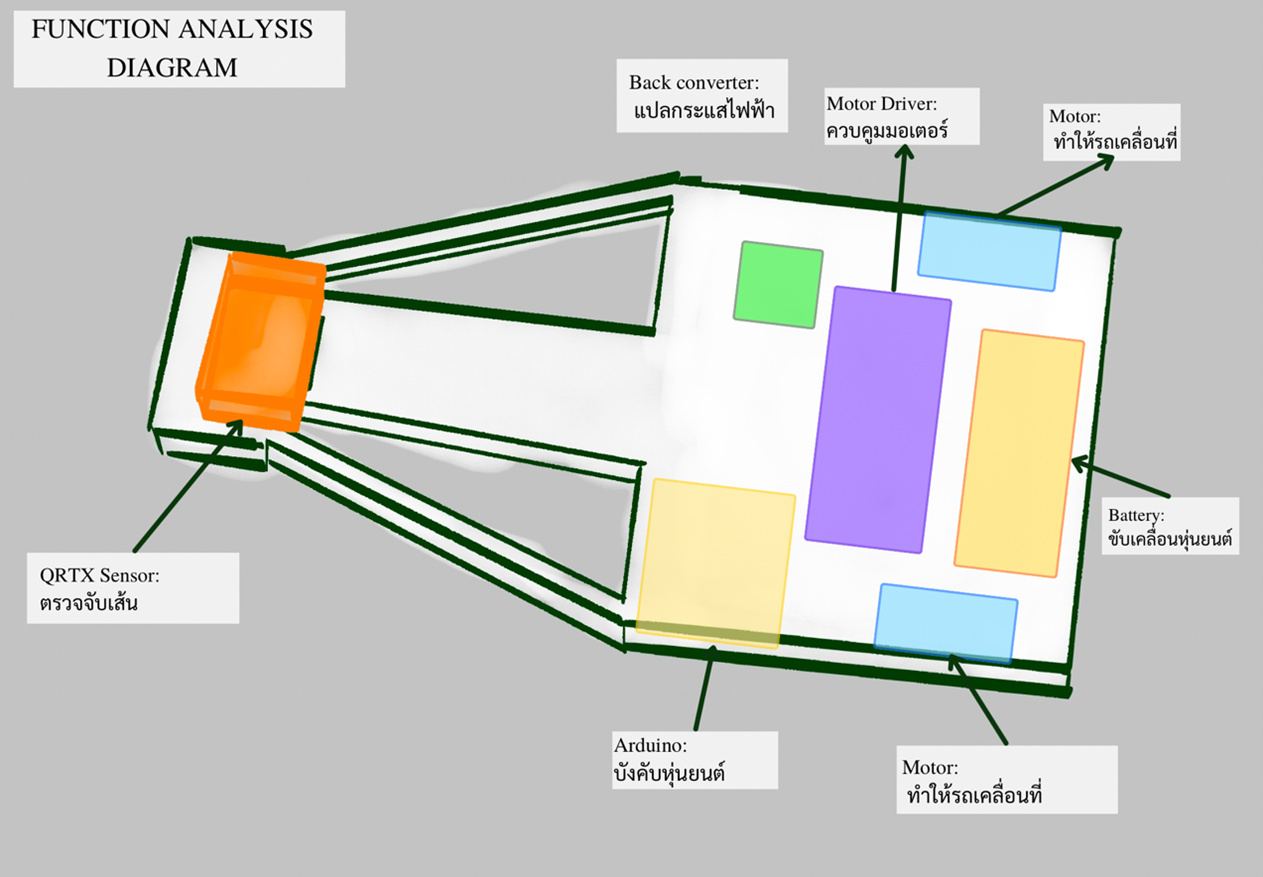
\includegraphics[width=415pt, height=288pt]{images/FunctionalAnalysisDiagram.png}
			\end{figure}
	\end{enumerate}
	ร่างโมเดลชิ้นงานแรก
	\begin{figure}[H]
		\centering
		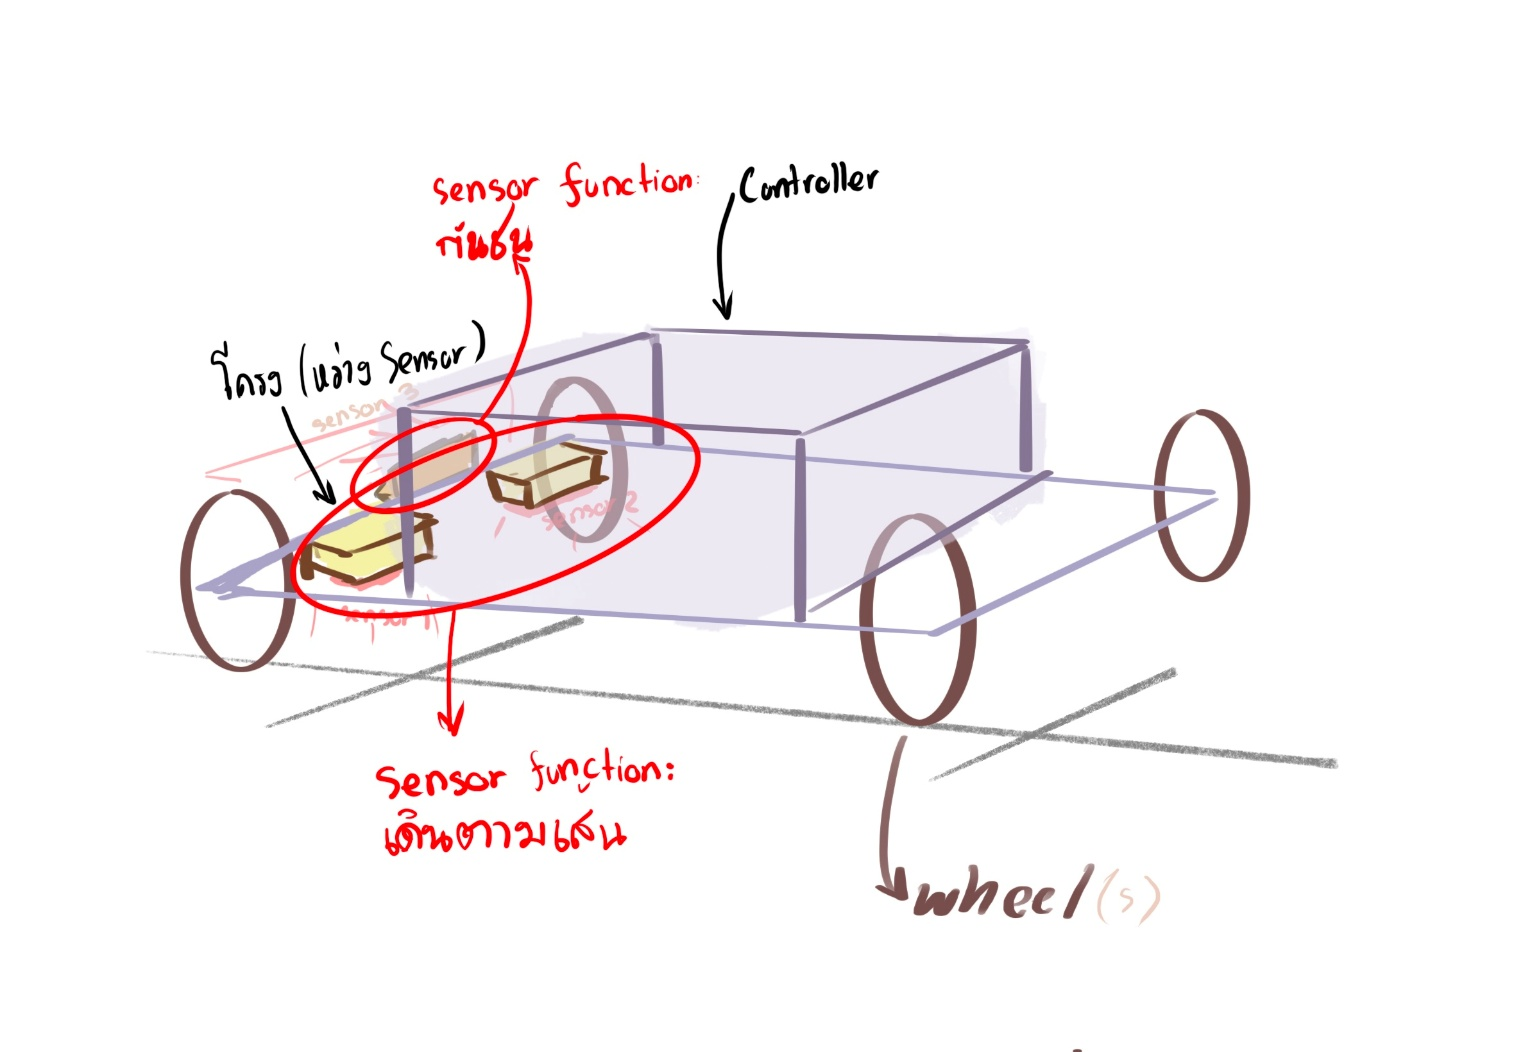
\includegraphics[width=415pt, height=288pt]{images/FirstDraft.jpeg} %300, 200
	\end{figure}
	\item วางแผนและดำเนินการแก้ปัญหา
	\begin{enumerate}
		\item ประกอบหุ่นยนต์ 
		\begin{enumerate}
			\item ตั้งให้ฐานหันด้านบนขึ้น เอา Buck Converter ต่อกับฐานโดยหันด้านบนขึ้นและใช้ไขควงขันสกรู M2 เชื่อมโดยแนะนำให้ขันผ่านรูของตัวแปลงกระแสลงผ่านรูบนฐานตำแหน่งที่ 9 และ 10 จำนวน 2 ตำแหน่ง, เอามอเตอร์ 2 ตัวซ้ายขวาของรถต่อกับฐานโดยใช้ตัว Motor brackets เป็นตัวยึดแล้วยึด Motor brackets กับฐานอีกที โดยหันมอเตอร์ด้านเพลาออกนอกรถ ยึด Motor brackets โดยใช้ไขควงขันสกรู M2 เชื่อมผ่านรูบน Motor  Brackets ลงไปผ่านรูบนฐานตำแหน่งที่ 11 และ 12 สำหรับมอเตอร์ทางขวา และ 13 และ 14 สำหรับมอเตอร์ทางซ้าย, เชื่อมเซ็นเซอร์กับฐานโดยพลิกฐานให้ด้านล่างหงายขึ้นแล้ววาง QTRX-MD-08A Reflectance Sensor Array แบบหันด้านที่มีชุด Sensors ขึ้นแล้วใช้ไขขวงขันสกรู M2 จากรูของ QTRX-MD-08A Reflectance Sensor Array ลงผ่านรูของฐานตำแหน่ง 1 และ 2 จากนั้ันพลิกฐานกลับแล้วใส่น๊อตไว้ด้านบนฝั่งละสองอีกที, เอา Ball Caster เชื่อมกับฐานโดยพลิกเอาด้านล้างขึ้นจากนั้นใช้ไขควงขันสกรู M2 ขันผ่านรูของฐาน Ball Caster ลงไปผ่านรูของฐานตำแหน่ง 3 และ 4 พลิกฐานกลับและเอาเบดบอร์ด 2 อัน เชื่อมกับฐานโดยต่อด้านบนวางติดกันบริเวณพื้นที่ว่างทางซ้ายและใช้ไขควงขันสกรูผ่านรูเบดบอร์ดลงไปในเนื้อของฐาน
			\item ใช้มือหัก Header แบบตรงให้เหลือ 8 pins จำนวน 1 แท่ง 6 pins จำนวน 1 แท่ง และใช้มือหัก Header แบบเฉียง 90 องศาให้เหลือ 11 pins จำนวน 1 แท่ง
			\item นำ Header แบบตรงจำนวน 8 pins ที่หักไว้เสียบด้าน pin ยาวเสียบที่ breadboard โดยเสียบแนวตามยาวของเบรดบอร์ด(ไม่ให้แต่ละพินเชื่อมกัน) เว้นระยะและนำ Header แบบตรงจำนวน 6 pins ที่หักไว้ตัวที่สองเสียบห่างจาก Header อันแรก 5 ช่องเบรดบอร์ด (นับช่องถัดจาก Header อันแรกเป็นที่หนึ่ง (ถ้า breadboard มีที่ว่าง (ไม่มีช่องพิน) ให้ประมาณช่องพินโครงงานนี้ประมาณได้ 2 ช่องพิน)และนับต่อไปเรื่อยๆแล้วใส่ Header ตัวที่สองที่ช่องที่ 5 ให้ขนานกับ Header อันแรก) โดยให้ Header 6 pins ห่างจากตัวสังเกตมากกว่า Header 8 pins แล้วนำ TB6612FNG Dual Motor Driver Carrier วางบน Headers ทั้งสองโดยหันด้านบนขึ้น และ Headers ที่เสียบไว้เข้ากับช่องพินของ TB6612FNG Dual Motor Driver Carrier ฝั่งตรงข้ามกับฝั่งที่มีช่องที่ต่อกับมอเตอร์โดยตรงครบทุกช่องพอดีแล้วอีกฝั่งจะมีช่อง VMOT และ GND เพียงสองช่องที่ไม่ถูกเสียบกับ Header 6 พินแล้วบัดกรีทุกพินของ Header เข้ากับช่องของ TB6612FNG Dual Motor Driver Carrier ทุกพิน และนำสายไฟ XT60-JST 28WG ที่ปลอกปลายด้าน JST ออก (โดยใช้ Flush Cutter) และบัดกรีปลายที่ปลอกออกเข้ากับ pin VMOT (แนะนำให้บักกรีเข้ากับสายสีแดง) และ GND (แนะนำให้บักกรีเข้ากับสายสีดำ)
			\item นำ Header แบบเฉียง 90 11 pins ไปบักกรีเข้ากับ QTRX-MD-08A Reflectance Sensor Array โดยต้องเสียบเข้ากับช่อง QTRX-MD-08A Reflectance Sensor Array ครบทุกช่อง
			\item บัดกรี XT60-JST 28WG ด้านที่ปลอกปลายด้าน JST ออก (โดยใช้ Flush Cutter) เข้ากับ pin ไฟเข้าขั้วบวก (แนะนำให้บักกรีเข้ากับสายสีแดง) และ ขั้วลบ (แนะนำให้บักกรีเข้ากับสายสีดำ) และเชื่อมหัว XT60 กับ ปลายสายแยก XT60 Splitter และบัดกรีสาย Jumper ด้านที่ปลอกสายออกเข้ากับ pin ไฟออกขั้วบวก (แนะนำให้บักกรีเข้ากับสายสีแดง) และ ขั้วลบ (แนะนำให้บักกรีเข้ากับสายสีดำ) โดยอีกฝั่งเป็นตัวผู้แล้วเสียบเข้า Breadboard ที่เขื่อมกับ pins VIN (ขั้วบวก) และ GND (ขั้วลบ)
			\item บัดกรีสาย Jumper ด้านที่ปลอกออก (โดย Flush Cutter) เข้ากับสายมอเตอร์ทั้งสองมอเตอร์ (แนะนำให้ใช้สีดำและแดงเพราะจะได้แยกขั้วบวกและลบได้ง่าย และให้หัวสาย Jumper อีกด้านเป็นตัวผู้เพื่อจะได้เสียบกับเบดบอร์ดได้โดยตรงแต่โครงงานนี้ใช้หัวตัวเมีย (แค่สำหรับมอเตอร์จำนวนสองคู่) แล้วใช้สาย Jumper ผู้-ผู้ เสียบกับตัวเมียเปลี่ยนให้ปลายสุดเป็นตัวผู้เพราะสาย Jumper ของมอเตอร์มีหัวตัวเมียเท่านั้น
เ			\item ชื่อมสาย Jumper กับ QTRX-MD-08A Reflectance Sensor Array:
				\begin{enumerate}
					\item เสียบหัวตัวผู้เข้ากับเบดบอร์ดที่เชื่อมกันกับ Pin D9 ของ Arudino nano esp32 และต่อหัวตัวเมียเข้ากับ Header ที่เชื่อมกับ Pin ODD ของ QTRX-MD-08A Reflectance Sensor Array
        			\item เสียบหัวตัวผู้เข้ากับเบดบอร์ดที่เชื่อมกันกับ Pin 3.3V และ GND ของ Arudino nano esp32 และต่อหัวตัวเมียเข้ากับ Header ที่เชื่อมกับ Pin VCC และ GND ตามลำดับของ QTRX-MD-08A Reflectance Sensor Array
            		\item เสียบหัวตัวผู้เข้ากับเบดบอร์ดที่เชื่อมกันกับ Pin A0 ถึง A7 ของ Arudino nano esp32 และต่อหัวตัวเมียเข้ากับ Header ที่เชื่อมกับ Pin 1,3,5,7,9,11,13,15 ของ QTRX-MD-08A Reflectance Sensor Array (แนะนำให้เชื่อมตามลำดับและใช้สาย Jumper ที่เชื่อมกันระหว่างสายเป็นพวงแล้วฉีกออกเป็นกลุ่มตามจำนวนที่ต้องการเพื่อความง่ายและสะดวกสบาย)
				\end{enumerate}
			\item เชื่อมสาย Jumper กับ TB6612FNG Dual Motor Driver Carrier: 
			\begin{enumerate}
				\item เสียบหัวตัวผู้เข้ากับเบดบอร์ดที่เชื่อมกันกับ Pin D8 ถึง GND ของ Arudino nano ESP32 และต่อหัวตัวผู้เข้ากับเบดบอร์ดที่เชื่อมกันกับ Pin PWMA, AIN2, AIN1, STBY, BIN1, BIN2, PWMB และ GND ของ TB6612FNG Dual Motor Driver Carrier (แนะนำให้เชื่อมตามลำดับและใช้สาย Jumper ที่เชื่อมกันระหว่างสายเป็นพวงแล้วฉีกออกเป็นกลุ่มตามจำนวนที่ต้องการเพื่อความง่ายและสะดวกสบาย)
				\item เสียบหัวตัวผู้เข้ากับเบดบอร์ดที่เชื่อมกันกับ Pin 3.3V และ GND ของ Arudino nano ESP32 และต่อหัวตัวผู้เข้ากับเบดบอร์ดที่เชื่อมกันกับ Pin VCC และ GND ของ TB6612FNG Dual Motor Driver Carrier
				\item เชื่อมหัว XT60 ที่เชื่อมกับ pins VMOT และ GND เข้ากับ XT60 Splitter
				\item เสียบหัวตัวผู้เข้ากับ pin AO1, AO2, BO1, BO2 ของ TB6612FNG Dual Motor Driver Carrier โดยโครงงานนี้เลือกเชื่อม AO1 และ AO2 กับมอเตอร์ด้านซ้าย และ BO1 และ BO2 กับมอเตอร์ด้านขวา (มอเตอร์ซ้าย-ขวาและสายในมอเตอร์เดียวกันสามารถสลับกันได้)
			\end{enumerate}
			\item เชื่อม XT60 ปลายรวมกับ LiPo 2S 7.4V 850 mAh เป็นการจ่ายไฟให้หุ่นยนต์เครื่อนที่ เป็นอันเสร็จ \\
			1.	ออกแบบเขียนโปรแกรม: เขียนโปรแกรมของระบบต่างๆของหุ่นยนต์เช่นระบบเดินตามเส้นของหุ่นยนต์,  
			ระบบเซนเซอร์กันชน เป็นต้น \\
			สรุปและรายงานผล: รายงานผลลัพธ์ และข้อสรุปต่างๆหน้าห้องเรียน 

			\textit{Source Code หุ่นยนต์} \url{https://github.com/arckanop/LineFollowing-Robot/blob/f862928533939fccaafa981bf8559cdd47ef3958/src/LineFollower/main.c%2B%2B}
		\end{enumerate}
	\end{enumerate}
	\item ทดสอบประเมินผลและปรับปรุงแก้ไข \\
	การทดลองหาความคลาดเคลื่อนของหุ่นยนต์โดยการใช้ความเร็วที่แตกต่างกัน \\
	\textbf{ตัวแปรในการทดลอง (ในสนามแต่ละแบบ)} \\
	\textbf{ตัวแปรต้น} \\
	\indent ค่า Kp Ki Kd \\
	\textbf{ตัวแปรตาม} \\
	\indent การหลุดออกจากเส้น \\
	\indent การสั่นของรถ \\
	\indent ความเร็วในการเลี้ยว \\
	\textbf{ตัวแปรควบคุม} \\
	\indent ตำแหน่งและจำนวนเซนเซอร์ \\
	\indent ความสว่าง \\
	\indent สถานที่ในการทดลอง \\
	\indent รูปแบบการเคลื่อนที่ \\[0.3em]
	\textbf{ออกแบบการทดลอง} \\
	การทดลองนี้เป็นการทดลองเพื่อหาค่า Kp Ki Kd ที่แตกต่างกัน เพื่อหาค่าที่เหมาะสมที่สุดในการใช้ใน 
PID Control โดยเริ่มหาที่ละค่า Kp Ki Kd ตามลำดับ โดยเริ่มแรกจะกำหนดให้ Ki และ Kd = 0 เพื่อหาค่า Kp ที่เหมาะสม เมื่อได้ค่า Kp ที่เหมาะสมแล้วจึงจะทำการทดลองหาค่า Ki โดยใช้ค่า Kp ที่เหมาะสมที่สุด และใช้   Kd = 0 เมื่อได้ Ki ที่เหมาะสมแล้วจึงจะหาค่า Kd โดยการใช้ Kp และ Ki เหมาะสมที่สุดโดยมีรูปแบบการเคลื่อนที่ที่ใช้ทดสอบค่า Kp Ki Kd ที่เหมาะสมดังภาพ \\

\begin{figure}[H]
	\centering
	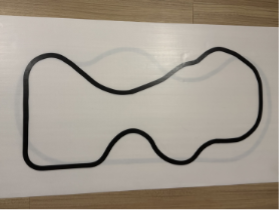
\includegraphics[width=210pt, height=160pt]{images/Track.png}
\end{figure}

ตารางแสดงผลการทดลอง
ค่า Kp (Ki = 0 Kd = 0)

\begin{table}[]
\begin{tabular}{|c|c|c|c|c|c|}
\hline
\textbf{ค่าที่ใส่} & 0.02 & 0.04 & 0.06 & 0.065 & 0.07 \\ \hline
ผลการเคลื่อนที่ & หลุดออกจากเส้น & หลุดออกจากเส้น & สั่นปานกลาง & ไม่สั่น/สั่นเล็กน้อย & สั่น \\ \hline
\end{tabular}
\end{table}

\begin{table}[]
\begin{tabular}{|l|l|l|l|l|l|}
\hline
\textbf{ค่าที่ใส่} & 0.04 & 0.06 & 0.075 & 0.09 & 0.11 \\ \hline
ผลการเคลื่อนที่ & \begin{tabular}[c]{@{}l@{}}การเลี้ยวเกิด\\    \\ ช้ามาก\end{tabular} & การเลี้ยวเกิดช้า & เกิดการเลี้ยวได้ปกติ & เกิดการเลี้ยวได้ช้าเล็กน้อย & \begin{tabular}[c]{@{}l@{}}การเลี้ยวเกิด\\    \\ ช้ามาก\end{tabular} \\ \hline
\end{tabular}
\end{table}

\indent จากการทดลอง พบว่าการใส่ค่า Ki ได้แก่ 0.02 0.04 0.06 0.08 0.09 0.10 0.11 ทำให้หุ่นยนต์หลุดออกจากเส้นในระหว่างการเคลื่อนที่ทั้งหมด \\
\indent จากการทดลองจึงสามารถสรุปได้ว่า ค่า Kp Ki Kd ที่เหมาะสมกับการใช้ใน PID Control ในการเคลื่อนที่ของหุ่นยนต์เดินตามเส้นในการทดลองนี้ ได้แก่ Kp = 0.065 Ki = 0 Kd = 0.075 \\[0.5em]

\textbf{ข้อเสนอแนะ} \\
ในการทดลองนี้กำหนด Ki = 0 ตลอด ซึ่งช่วยให้ระบบตอบสนองเร็ว แต่ยังอาจมี error คงค้าง (steady-state error) ได้ ในอนาคตควรทดลองเพิ่มค่า Ki ทีละน้อยเพื่อดูผลต่อความแม่นยำของการเดินตามเส้น

\end{enumerate}

\section*{แผนปฏิบัติงาน}
\begin{table}[]
\begin{tabular}{|l|l|llllllll|}
\hline
\multicolumn{1}{|c|}{\multirow{2}{*}{\textbf{กิจกรรม}}} & \multicolumn{1}{c|}{\multirow{2}{*}{\textbf{ผู้รับผิดชอบ}}} & \multicolumn{8}{c|}{\textbf{เดือน}} \\ \cline{3-10} 
\multicolumn{1}{|c|}{} & \multicolumn{1}{c|}{} & \multicolumn{1}{c|}{\textbf{ก.ค.}} & \multicolumn{1}{c|}{\textbf{ส.ค.}} & \multicolumn{1}{c|}{\textbf{ก.ย.}} & \multicolumn{1}{c|}{\textbf{ต.ค.}} & \multicolumn{1}{c|}{\textbf{พ.ย.}} & \multicolumn{1}{c|}{\textbf{ธ.ค.}} & \multicolumn{1}{c|}{\textbf{ม.ค.}} & \multicolumn{1}{c|}{\textbf{ก.พ.}} \\ \hline
ระดมความคิดและประชุมกลุ่ม & ทุกคน & \multicolumn{1}{l|}{} & \multicolumn{1}{l|}{/} & \multicolumn{1}{l|}{} & \multicolumn{1}{l|}{} & \multicolumn{1}{l|}{} & \multicolumn{1}{l|}{} & \multicolumn{1}{l|}{} &  \\ \hline
ค้นหาข้อมูลและสั่งอุปกรณ์ & ทุกคน & \multicolumn{1}{l|}{} & \multicolumn{1}{l|}{} & \multicolumn{1}{l|}{/} & \multicolumn{1}{l|}{/} & \multicolumn{1}{l|}{} & \multicolumn{1}{l|}{} & \multicolumn{1}{l|}{} &  \\ \hline
ออกแบบหุ่นยนต์ & 4,11,18 & \multicolumn{1}{l|}{} & \multicolumn{1}{l|}{} & \multicolumn{1}{l|}{} & \multicolumn{1}{l|}{} & \multicolumn{1}{l|}{/} & \multicolumn{1}{l|}{/} & \multicolumn{1}{l|}{/} &  \\ \hline
ประกอบหุ่นยนต์ & 18,25,39 & \multicolumn{1}{l|}{} & \multicolumn{1}{l|}{} & \multicolumn{1}{l|}{} & \multicolumn{1}{l|}{} & \multicolumn{1}{l|}{} & \multicolumn{1}{l|}{/} & \multicolumn{1}{l|}{/} &  \\ \hline
ทำการออกแบบระบบและเขียนโปรแกรม & 18,25 & \multicolumn{1}{l|}{} & \multicolumn{1}{l|}{} & \multicolumn{1}{l|}{} & \multicolumn{1}{l|}{} & \multicolumn{1}{l|}{} & \multicolumn{1}{l|}{} & \multicolumn{1}{l|}{} & / \\ \hline
ทดสอบการทำงานและปรับปรุงแก้ใข & 18,24,25,26 & \multicolumn{1}{l|}{} & \multicolumn{1}{l|}{} & \multicolumn{1}{l|}{} & \multicolumn{1}{l|}{} & \multicolumn{1}{l|}{} & \multicolumn{1}{l|}{} & \multicolumn{1}{l|}{} & / \\ \hline
สรุปและรายงานผล & ทุกคน & \multicolumn{1}{l|}{} & \multicolumn{1}{l|}{} & \multicolumn{1}{l|}{} & \multicolumn{1}{l|}{} & \multicolumn{1}{l|}{} & \multicolumn{1}{l|}{} & \multicolumn{1}{l|}{} & / \\ \hline
\end{tabular}
\end{table}
\section*{ผลที่คาดว่าจะได้รับ} \vspace{-1.25em}
\begin{enumerate}
	\item ระบบการทำงานของ PID Controller ถูกนำไปประยุกต์ใช้่กับหุ่นยนต์อื่นๆได้จริงอย่างมีประสิทธิภาพ
	\item หุ่นยนต์เดินตามเส้นพื้นฐานได้
	\item หุ่นยนต์เดินตามเส้นที่สามารถอธิบายการทำงานของ PID Controller และ Fast Fourier Transform ได้อย่างชัดเจน และทำงานได้ตามทฤษฏี
\end{enumerate}
\vspace{-0.5em}

\section*{แหล่งอ้างอิง} \vspace{-1.25em}
\begin{enumerate}[label={[{\arabic*}]}]
    \item J.~Ringwood and A.~O’Dwyer, “A frequency domain based self-tuning PID controller,” in \textit{Proc. Asian Control Conf.}, Tokyo, Japan, Jul. 1994, pp. 331–334. [Online]. Available: \url{https://mural.maynoothuniversity.ie/id/eprint/9538/} [Accessed: Sep.~1, 2025].

    \item R.~M.~Murray, “CDS 101/110: PID Control,” lecture notes, California Institute of Technology, Nov. 3, 2004. [Online]. Available: \url{https://www.cds.caltech.edu/~murray/courses/cds101/fa04/caltech/am04_ch8-3nov04.pdf} [Accessed: Sep.~1, 2025].

    \item X.~Chen, C.~Wang, and H.~Wu, “PID Controllers Parameters Self-Tuning Algorithm Based on Frequency Characteristic,” in \textit{2010 International Conference on Measuring Technology and Mechatronics Automation}, Changsha, China, 2010, pp. 891–894, doi: \url{10.1109/ICMTMA.2010.511}.

    \item M.~Benrabah, K.~Kara, O.~AitSahed, and M.~L.~Hadjili, “Adaptive Fourier Series Neural Network PID Controller,” \textit{International Journal of Control, Automation and Systems}, vol.~19, no.~10, pp.~3388–3399, Oct.~2021, doi: \url{10.1007/s12555-020-0185-3}.

    \item R.~McMenemy, “Implementing PID Control with Arduino and Fast Fourier Transform for Noise Reduction,” \textit{Medium}, Aug. 11, 2024. [Online]. Available: \url{https://rabmcmenemy.medium.com/implementing-pid-control-with-arduino-and-fast-fourier-transform-for-noise-reduction-0ab09c177f3d} [Accessed: Sep.~1, 2025].

    \item “Fourier Analysis Unlocks Powerful PID Control Secrets | ESP32 Reveals the Hidden Root Cause!,” \textit{SaludPCB}, Jun. 22, 2025. [Online]. Available: \url{https://saludpcb.com/pid-control-esp32-fourier-reveal/} [Accessed: Sep.~1, 2025].

    \item L.~Eitel, “PID design using frequency-domain methods,” \textit{Linear Motion Tips}. [Online]. Available: \url{https://www.linearmotiontips.com/pid-design-using-frequency-domain-methods/} [Accessed: Sep.~1, 2025].

    \item “Fourier Series and Fourier Transform – Lesson 3,” \textit{YouTube}, [Online Video]. Available: \url{https://www.youtube.com/watch?v=Ils6b1Y4W1U} [Accessed: Sep.~2, 2025].
\end{enumerate}

\section*{ภาพประกอบการทำโครงงาน}

\begin{center}
	ภาพประกอบการทำโครงงานและ Component Option Table ฉบับเต็มดูในภาคผนวก 
\end{center}

\end{document}

% \subsection*{ขั้นตอนการดำเนินงาน}
% \begin{adjustwidth}{2em}{0em}
% 	\begin{enumerate}
% 		\item ระดมความคิด: สมาชิกทุกคนวางแผนรายละเอียดต่างๆคร่าวๆ เช่น เลือกอุปกรณ์ที่ต้องใช้
% 		\item ออกแบบหุ่นยนต์: ออกแบบรูปร่างภายนอกของหุ่นยนต์ และตำแหน่งอุปกรณ์ต่างๆ เช่นตำแหน่งเซนเซอร์ 
% 		\item ออกแบบเขียนโปรแกรม: เขียนโปรแกรมของระบบต่างๆของหุ่นยนต์เช่นระบบเดินตามเส้นของหุ่นยนต์, ระบบเซนเซอร์กันชน เป็นต้น
% 		\item ทดสอบการทำงาน: อัปโหลดโปรแกรมและทดสอบการทำงานของหุ่นยนต์เดินตามเส้นโดยการให้หุ่นยนต์เดินตามเส้นที่กำหนดและสังเกตผล
% 		\item ปรับปรุงแก้ไข: แก้ไขข้อผิดพลาดที่เกิดขึ้นในขั้นตอนการทดสอบ (ถ้ามี) 
% 		\item สรุปและรายงานผล: รายงานผลลัพธ์ และข้อสรุปต่างๆหน้าห้องเรียน
% 	\end{enumerate}
% \end{adjustwidth}

% \subsection*{การรวบรวมข้อมูล}
% หาข้อมูลหัวข้อต่างๆ ได้แก่ \vspace{-0.5em}

% \begin{adjustwidth}{2em}{0em}
% 	\begin{enumerate}
% 		\item ทฤษฏีการทำงานของระบบ PID
% 		\item ทฤษฎีการทำงานของ Fast Fourier Transform (FFT)
% 		\item การทำงานหุ่นยนต์ (Workflow ของ PID Line Follower)
% 		\item การต่อวงจร
% 		\item ส่วนประกอบของหุ่นยนต์
% 			\begin{itemize}[leftmargin = 1em]
% 				\item Microcontroller - Arduino Nano ESP32
% 				\item Sensors - QTRX-MD-08A
% 				\item Motors - N20 Micrometal Gear Motor
% 				\item Motor Driver - TB6612FNG
% 				\item ล้อรถ
% 				\item โครงรถ
% 				\item แบตเตอรี่ - LiPo Battery
% 				\item สายไฟ - สาย Jumper
% 			\end{itemize}
% 	\end{enumerate}
% \end{adjustwidth}

% \subsection*{โครงงาน/งานวิจัยที่เกี่ยวข้อง}
% \vspace{-0.5em}
% \begin{adjustwidth}{2em}{0em}
% 	\indent \textbf{โครงงาน/งานวิจัยเกี่ยวกับระบบ PID}
% 	\begin{itemize}
% 		\item Chen et al., 2010 — Self-Tuning PID จากคุณลักษณะความถี่
% 		\item Benrabah et al., 2021 — AFSNNPID (Adaptive Fourier-Series Neural-Network PID)
% 		\item Ringwood \& O’Dwyer, 1994 — Frequency Domain Based Self-Tuning PID
% 	\end{itemize}

% 	\indent \textbf{โครงงาน/งานวิจัยเกี่ยวกับหุ่นยนต์เดินตามเส้น}
% 	\begin{itemize}
% 		\item Mehran pakdaman, M. Mehdi Sanaatiyan, Mahdi Rezaei Ghahroudi, 2010 — A Line Follower Robot from design to Implementation: Technical issues and problems
% 		\item Theunis R. Botha* and P. Schalk Els, 2019 — Vehicle centre of mass, roll-centre and pitch-centre height estimation
% 		\item Onur Erbay, Abdullah Burhan Doğan, Enes Devecioğlu, 2024 — Line Follower Robot with PID Control
% 	\end{itemize}
% \end{adjustwidth}